%version of 03-10-20

\chapter{Arithmetic: Putting Numbers to Work}
\label{ch:arithmetic}



\noindent
Previous chapters have given us sets, numbers, and numerals, the simple objects that we use to count and measure and aggregate.  The current chapter is devoted to expounding the rules of {\em arithmetic}, the system which allows us to manipulate these objects and to develop complicated objects out of the simple ones.

\section{The Basic Arithmetic Operations}
\label{sec:Arithmetic-Tools}
\index{laws of arithmetic}

The basic tools of arithmetic consist of a small set of operations on numbers/numerals, together with two special integers which play important roles with respect to the operations.  Since these entities, the operations and special numbers, are so tightly intertwined, we discuss them simultaneously.

\smallskip


\index{arithmetic!the arithmetic identities, $0$ and $1$} 
\index{number!zero ($0$), the additive identity} 
\index{number!one ($1$), the multiplicative identity}
\index{$0$: the additive identity} 
\index{$1$: the multiplicative identity}

\noindent {\small\sf The two special integers.}
The integers zero ($0$)  and one ($1$), play special roles as the tools of arithmetic are applied to all four classes of numbers described in Chapter~\ref{ch:numbers-numerals}.

\smallskip

\index{arithmetic!basic operations}

\noindent {\small\sf The operations of arithmetic.}
Arithmetic on the classes of numbers described in Chapter~\ref{ch:numbers-numerals} is built upon a rather small repertoire of operations.  When we say that an operation produces a number ``of the same sort'', we mean that it produces:
\begin{itemize}
\item
an integer result from integer arguments;
\item
a rational (number) result from rational (number) arguments;
\item
a real (number) result from real (number) arguments;
\item
a complex (number) result from complex (number) arguments.
\end{itemize}
The fundamental operations on numbers are, of course, familiar to the reader.  Our goal in discussing them is to stress the laws that govern the operations.  Along the way, we also introduce a few operations that are less familiar but no less important.

\subsection{Unary (Single-Argument) Operations}
\label{sec:unary-ops}

\subsubsection{Negating and reciprocating numbers}
\index{arithmetic!basic operations!negation}
\index{arithmetic!basic operations!negating} \index{number!negative}

\noindent {\it i. The operation of {\em negation}}:
\begin{itemize}
\item
is a {\em total function} on the sets $\Z, \Q, \R, \C$.  It replaces a number $a$ by its {\em negative}, which is a number of the same sort.

\smallskip

The {\it negative} of a number $a$ is denoted $-a$ and is usually articulated ``minus $a$'' or ``negative $a$''.
\item
is a {\em partial function} on the nonnegative subsets of $\Z, \Q, \R, \C$.  It replaces a number $a$ by its negative, $-a$, whenever both $a$ and $-a$ belong to the nonnegative subset being
operated on.
\end{itemize}
Zero ($0$) is the unique {\it fixed point} of the operation, meaning that $0$ is the unique number $a$ such that $a = -a$.
\index{function!fixed point}\index{arithmetic!negation!fixed point}

\medskip

\index{arithmetic!basic operations!reciprocal}
\index{arithmetic!basic operations!reciprocating} \index{number!reciprocal}

\noindent {\it ii. The operation of {\em reciprocation}}:
\begin{itemize}
\item
is a {\em total function} on the sets $\Q, \R, \C$, which replaces each number $a$ by its {\em reciprocal}, a number of the same sort.

\smallskip

The {\it reciprocal} of  a number $a$ is denoted $1/a$ or $\displaystyle {1 \over a}$; we shall employ whichever notation enhances legibility.  It is usually articulated ``$1$ over $a$''.

\item
is {\em undefined} on every integer $a$ except for $a=1$.
\end{itemize}

\subsubsection{Floors, ceilings, magnitudes}
\index{arithmetic!basic operations!floor}
\index{arithmetic!basic operations!ceiling}
\index{arithmetic!basic operations!absolute value}
\index{arithmetic!basic operations!magnitude}

\index{arithmetic!basic operations!integer part of a number}
\index{arithmetic!basic operations!floor of a number}
\noindent {\it i. The operations of {\em taking floors and ceilings}}
are total operations on the sets $\N, \Z, \Q, \R$.
\begin{itemize}
\item
The {\it floor} of a number $a$, also called {\it the integer part} of $a$, is denoted $\lfloor a \rfloor$.  It is the largest integer which does not exceed $a$; i.e.,:
\[
\lfloor a \rfloor \ \eqdef \ \max_{b \in {\mathbb{N}}} \Big[ b \ \leq a \Big]
\]
\item
The {\it ceiling} of a number $a$ of $a$, denoted $\lceil a \rceil$, is the smallest integer which is 
not smaller than $a$:
\[
\lceil a \rceil \ \eqdef \ \min_{b \in {\mathbb{N}}} \Big[ b \ \geq a \Big]
\]
\end{itemize}
The operations of taking floors and ceilings are two common ways to {\em round} rationals and reals to their ``closest'' integers.
\index{arithmetic!basic operations!ceiling of a number}
\index{arithmetic!basic operations!rounding to ``closest'' integer}

\medskip

\index{arithmetic!basic operations!absolute value, magnitude}
\noindent {\it ii. The operations of taking {\em absolute values/magnitudes}}:
Let $a$ be a real number.  The {\it absolute value}, or, {\it magnitude}, of $a$, denoted $|a|$ equals either $a$ or $-a$, whichever is positive.  For a complex number $a$, the definition of
$|a|$ is more complicated: it is a measure of $a$'s ``distance'' from the ``origin'' complex number $0 + 0 \cdot i$.  In detail:
\[
|a| \ = \ \left\{
\begin{array}{cl}
a & \mbox{ if } \ \big[a \in \R \big] \ \ \mbox{ and } \ \ \big[a \geq 0\big] \\
-a & \mbox{ if } \ \big[a \in \R\big] \ \ \mbox{ and } \ \ \big[a < 0\big] \\
\sqrt{b^2 + c^2} &  \mbox{ if } \ \big[a \in \C\big]  \ \ \mbox{ and }  \ \ \big[a = (b+ci)\big]
\end{array}
\right.
\]

\subsubsection{Factorials (of a nonnegative integer)}
\index{arithmetic!basic operations!factorial (of a nonnegative integer)}

\index{arithmetic!basic operations!$n!$: factorial of $n \in \N$}

The {\it factorial} of a nonnegative integer $n \in \N$, which is commonly denoted $n!$, is the function defined via the following recursion.
\begin{equation}
\label{eq:n-factorial-recursion}
\mbox{\sc fact}(n) \ = \ \left\{
\begin{array}{cl}
1 & \mbox{  if } \ n=0 \\
n \cdot \mbox{\sc fact}(n-1) & \mbox{  if } \ n>0
\end{array}
\right.
\end{equation}
We can ``unwind'' the recursion in (\ref{eq:n-factorial-recursion}) and, thereby, derive an iterative expression for $n!$.  In what follows, we denote multiplication by the familiar symbol $\times$ rather than the centered dot ($\cdot$), to enhance legibility.  We find that, for all $n \in \N$,
\begin{equation}
\label{eq:n-factorial-direct}
n! \ = \ \mbox{\sc fact}(n) \ = \ 
n \times (n-1) \times (n-2) \times \cdots \times 2 \times 1
\end{equation} 
A $3$-step inductive argument validates this ``unwinding'':
\begin{enumerate}
\item
If $n =0$, then {\sc fact}$(n) = 1$, by definition (\ref{eq:n-factorial-recursion}).
\item
Assume, for induction, that the expansion in (\ref{eq:n-factorial-direct}) is valid for a given $k \in N$:
\[ \mbox{\sc fact}(k) \ = \ k \times (k-1) \times (k-2) \times \cdots \times 2 \times 1 \] 
\item
Then:
\[
\begin{array}{lclll}
\mbox{\sc fact}(k+1) & = & (k+1) \cdot \mbox{\sc fact}(k)
  & & \mbox{by (\ref{eq:n-factorial-recursion})} \\
  & = &
(k+1) \times k \times (k-1) \times (k-2) \times \cdots \times 2 \times 1
  & & \mbox{by induction}
\end{array}
\]
\end{enumerate}


\subsection{Binary (Two-Argument) Operations}
\label{sec:binary-operators}

\subsubsection{Addition and Subtraction}
\index{arithmetic!basic operations!addition} \index{arithmetic!basic operations!subtraction}
\index{arithmetic!addition}

The operation of {\it addition} is a {\em total function} which replaces any two numbers $a$ and $b$ by a number of the same sort.  The resulting number is the {\em sum of $a$ and $b$} and is denoted $a+b$.
\index{arithmetic!addition!sum}

\smallskip

\index{arithmetic!subtraction} \index{arithmetic!subtraction!difference}
\noindent
The operation of {\it subtraction} is a {\em total function} on the sets $\Z, \Q, \R, \C$, which replaces any two numbers $a$ and $b$ by a number of the same sort.  The resulting number is the {\em difference of $a$ and $b$} and is denoted $a-b$.  On the nonnegative subsets of the sets $\Z, \Q, \R, \C$---such as $\N$, which is the largest nonnegative subset of $\Z$---subtraction is a {\em partial function} which is defined only when $a \geq b$.

\smallskip

Subtraction can also be defined as follows.  For any two numbers $a$ and $b$, {\em the difference of $a$ and $b$ is the sum of $a$ and the negation of $b$}:
\[ a-b \ = \ a + (-b) \]

\medskip

\index{number!additive identity}
\index{number!identity under addition}\index{identity!additive}

\noindent {\em The special role of $0$ under addition and subtraction.}
The number $0$ is the {\it identity} under addition and subtraction; terminologically, $0$ is an {\it additive identity}.  This means that, for all numbers $a$,
\[ a+0 \ = \ a-0 \ = \ a. \]
One shows as follows that $0$ is {\em the} additive identity.

\begin{prop}
\label{thm:unique-add-iden}
The number $0$ is the unique additive identity.
\end{prop}

\begin{proof}
Assume, for contradiction, that there is an additional additive identity, call it $0'$.  By definition of ``additive identity'', we would then have
\[ 0 \ = \ 0 + 0' \ = \ 0' \]
It follows that all additive identities are equal, meaning that there is only one.  \qed
\end{proof}

\medskip

\noindent {\em The special role of $1$ under addition and subtraction.}
\index{arithmetic!integers!successor} \index{arithmetic!integers!predecessor}
For any integer $a$, there is no integer between $a$ and $a+1$ nor between $a-1$ and $a$. For this reason, on the sets $\Z$ and $\N$, one often singles out the following special cases of addition and subtraction, especially in reasoning about situations that are indexed by integers.  Strangely, these operations have no universally accepted notations.
\begin{itemize}
\item
The {\it successor} operation is a {\em total function} on both $\N$ and $\Z$, which replaces an
integer $a$ by the integer $a+1$.
\item
The {\it predecessor} operation is a {\em total function} on $\Z$, which replaces an integer $a$ by the integer $a-1$.  It is a {\em partial function} on $\N$, which is defined only when the argument $a$ is positive (so that $a-1 \in \N$).
\end{itemize}

\smallskip

\index{functional inverse}
The operations of addition and subtraction are {\em mutually inverse operations}, in the sense of the following definition.  Function $f$ is a {\it functional inverse} of function $g$ if for all arguments $x$,
\begin{equation}
\label{eq:functional-inverse}
f(g(x)) \ = \ x
\end{equation}
In suggestive terminology, applying function $f$ ``undoes'' the result of applying function $g$.  Within the current context, each of addition and subtraction is a functional inverse of the other, so that equation (\ref{eq:functional-inverse}) takes the following dual form.
\[ a \ = \ (a+b) -b \ = \ (a-b) +b \]
\index{arithmetic!integers!additive inverse} 
\index{arithmetic!integers!addition and subtraction are mutually inverse}

\subsubsection{Multiplication and Division}
\index{arithmetic!basic operations!multiplication} \index{arithmetic!basic operations!division}
\index{arithmetic!multiplication} \index{arithmetic!multiplication!product}
\index{arithmetic!multiplication!$a \cdot  b$} \index{arithmetic!multiplication!$a \times b$}

The operation of {\it multiplication} is a {\em total function} that replaces any two numbers $a$ and $b$ by a number of the same sort.  The resulting number is the {\em product of $a$ and $b$} and is denoted either $a \cdot b$  or $a \times b$.  We shall usually favor the former notation (to save space), except when the latter enhances legibility.

\smallskip

\index{arithmetic!division} \index{arithmetic!division!When is $a/b$ defined?}
\index{arithmetic!division!quotient} \index{arithmetic!division!quotient!${a \over b}$}
\index{arithmetic!division!quotient!$a/b$} \index{arithmetic!division!quotient!$a \div b$}

The operation of {\it division} is a {\em partial function} on all of our sets of numbers.  Given two numbers $a$ and $b$, the result of dividing $a$ by $b$---{\em when that result is defined}---is the {\it quotient of $a$ by $b$;} it is denoted by one of the following three notations:
\[  a/b, \ \ \ a \div b, \ \ \ {a \over b}  \]
The {\it quotient of $a$ by $b$} is defined precisely when {\em both}

\noindent
\hspace*{.35in}(1) $b \neq 0$: one can never divide by $0$ \\
\hspace*{.35in}{\em and} \\
\hspace*{.35in}(2) there exists a number $c$ such that $a = b \cdot c$

\noindent
Assuming that condition (1) holds, {\em condition (2) always holds when $a$ and $b$ belong to $\Q$ or $\R$ or $\C$}.

\smallskip

Division can also be defined as follows.  For any two numbers $a$ and $b$, {\em the quotient of $a$ and $b$ is the product of $a$ and the reciprocal of $b$} (assuming that the latter exists):
\[ a/b \ = \ a \times (1/b) \]
Computing reciprocals of nonzero numbers in $\Q$ and $\R$ is standard high-school level fare; computing reciprocals of nonzero numbers in $\C$ requires a bit of calculational algebra which we do not cover.  For completeness, we note that the reciprocal of the {\em nonzero} complex number $a + bi \in \C$ is the complex number $c+di$ where
\[ c \ = \ \frac{a}{a^2 + b^2} \ \ \ \ \
\mbox{ and } \ \ \ \ \
d \ = \ \frac{-b}{a^2 + b^2}
\]

\medskip

\index{number!multiplicative identity}
\index{number!identity under multiplication} \index{identity!multiplicative}

\noindent {\em The special role of $1$ under multiplication and division.}
The number $1$ is the {\it identity} under the operations of multiplication and division; terminologically, $1$ is a {\it multiplicative identity}.  This means that, for all numbers $a$,
\[ a \cdot 1 \ = \ a \cdot (1/1) \ = \ a \]
One shows as follows that $1$ is {\em the} multiplicative identity.

\begin{prop}
\label{thm:unique-mult-iden}
The number $1$ is the unique multiplicative identity.
\end{prop}

\begin{proof}
Assume, for contradiction, that there is an additional multiplicative identity, call it $1'$.  By definition of ``multiplicative identity'', we would then have
\[ 1 \ = \ 1 \times 1' \ = \ 1' \]
It follows that all multiplicative identities are equal.  \qed
\end{proof}

\medskip

\index{multiplicative annihilator}

\noindent {\em The special role of $0$ under multiplication and division.}
The number $0$ is the {\it annihilator} under multiplication.  This means that, for all numbers $a$
\[ a \times 0 \ = \ 0 \]
Using reasoning which parallels that of Propositions~\ref{thm:unique-mult-iden} and~\ref{thm:unique-mult-iden}, the reader can prove that $0$ is {\em the unique} multiplicative annihilator.

\begin{prop}
The number $0$ is the unique multiplicative annihilator.
\end{prop}

\medskip

\index{arithmetic!integers!multiplicative inverse}
\index{arithmetic!integers!multiplication and division are mutually inverse}

The operations of multiplication and division are mutually inverse operations, in the sense of equation (\ref{eq:functional-inverse}): each can be used to ``undo'' the other.
\[ a = (a \times b) \div b \ = \ (a \div b) \times b  \]

\subsubsection{Exponentiation and Taking Logarithms}
\label{sec:exponentiation}

\index{arithmetic!basic operations!exponentiation}
\index{arithmetic!raising a number to a power}

A conceptually powerful notational construct is the operation of {\it exponentiation},  i.e., {\it raising a number to a power}.  For real numbers $a$ and $b$, the {\it $b$th power} of $a$, denoted $a^b$ is defined by the system of equations
\begin{equation}
\label{eq:power-def}
\begin{array}{llll}
\mbox{for all numbers $a>0$} & & & a^0 = 1 \\
 & & & \\
\mbox{for all numbers $a, b, c$} & & & a^b \cdot a^c = a^{b+c}
\end{array}
\end{equation}
This deceptively simple definition has myriad consequences which we often take for granted.
\index{$a^{1/2}$: the square root of number $a$} \index{square root}
\index{$\sqrt{a}$: the square root of number $a$}
\begin{itemize}
\item
{\em Multiplication of exponentials is accomplished via addition within the exponents.}

\item
{\em For all numbers $a>0$, the number $a^0 = 1$}

\smallskip

This follows (via cancellation) from system (\ref{eq:power-def}) via the fact that
\[ a^b \cdot a^0 \ = \ a^{b+0} \ = \ a^b \ = \ a^b \cdot 1  \]

\item
{\em For all numbers $a >0$, the number $a^{1/2}$ is the {\it square root} of $a$; i.e., $a^{1/2}$ is the (unique, via cancellation) number $b$ such that $b^2 = a$.}
(Another common notation for the number $a^{1/2}$ is $\sqrt{a}$.)

\smallskip

This follows from system (\ref{eq:power-def}) via the fact that
\[ a \ = \ a^1 \ = \ a^{(1/2) + (1/2)} \ = \ a^{1/2} \cdot a^{1/2} \ = \ \left(a^{1/2}\right)^2. \]

\item
{\em For all numbers $a>0$ and $b$, the number $a^{-b}$ is the {\it multiplicative inverse} of $a^b$, meaning that $a^b \times a^{-b} = 1$}

\smallskip

This follows from system (\ref{eq:power-def}) via the fact that
\[ a^b \cdot a^{-b} \ = \ a^{(b + (-b))} \ = \ a^0 \ = \  1 \]
\end{itemize}
When the power $b$ is a positive integer, then definition (\ref{eq:power-def}) can be cast in the following attractive inductive form:
\begin{equation}
\label{eq:power-def-integer}
\begin{array}{llll}
\mbox{for all numbers $a>0$} & & & a^0 = 1 \\
 & & & \\
\mbox{for all numbers $a$ and integers $b$} & & & a^{b+1} = a \times a^b
\end{array}
\end{equation}

\medskip

We now have the background needed to manipulate and employ powers that are integral or fractional, positive, zero, or negative.

\bigskip

\noindent
Just as addition has its inverse operation, subtraction, and multiplication has its inverse operation, division, the operation of exponentiation has its inverse operation, {\it taking logarithms}.  Our main discussion of logarithms appears in Section~\ref{sec:exponential+logarithm}; we just define the operation here.

\medskip

\index{arithmetic!basic operations!taking logarithms}
For positive real numbers $a$ and $b$, the operation of taking logarithms is defined by the following dual equation.
\[ \log_b (b^a) \ = \ b^{\log_b a} \ = \ a \]
We shall note in Section~\ref{sec:exponential+logarithm} that most of the main properties of this operation can be inferred from properties of the operation of exponentiation.

\bigskip

\noindent \fbox{
\begin{minipage}{0.96\textwidth}
{\bf Explanatory note}.

We have remarked in several places about the importance of noticing patterns as we ``do'' mathematics.  A pattern that leads to some beneficial insights has emerged in the current section.  The pattern suggests that in certain senses:
\begin{itemize}
\item
The operations of addition, multiplication, and exponentiation ``behave'' similarly to one another.
\item
The operations of subtraction, division, and taking logarithms ``behave'' similarly to one another.
\item
The operations addition and subtraction relate to one another \\
\hspace*{.2in}in much the same way as \\
the operations multiplication and division relate to one another \\
\hspace*{.2in}and in much the same way as \\
the operations exponentiation and taking logarithms relate to one another.
\end{itemize}
This pattern is ``encoded'' by the following suggestive figure.
\[ 
\begin{array}{|ccccc|}
\hline
\mbox{addition}
  & \approx &
\mbox{multiplication}
  & \approx &
\mbox{exponentiation} \\
\updownarrow & &
\updownarrow & &
\updownarrow \\
\mbox{subtraction}
  & \approx &
\mbox{division}
  & \approx &
\mbox{taking logarithms} \\
\hline
\end{array}
\]

\smallskip

Of course, patterns are {\em de}scriptive rather than {\em pre}scriptive, so one must use them only as hints to be followed or as inspirations for further investigation, not as facts to be depended on.
\end{minipage}
}
\bigskip


\subsubsection{Binomial coefficients and Pascal's triangle}
\label{sec:binomial-coeff}
\index{arithmetic!basic operations!binomial coefficient}

We close our catalogue of arithmetic operations with a binary operation on the set $\N \times \N$\footnote{In advanced contexts, one encounters binomial coefficients with arguments which are either nonintegral or nonpositive.}~known as the {\it binomial coefficient}.  The versatility of this operation---and the origin of the unexpected word ``coefficient'' in its name---will become clear throughout our text.  We now lay the groundwork for the {\em many} applications of binomial coefficients.

%in Section~\ref{sec:Binomial-thm} and in
%Chapters~\ref{ch:Summation},~\ref{ch:Recurrences},
%and~\ref{ch:prob-stat}.

\medskip

\index{$n$ choose $k$: the binomial coefficient $\displaystyle {n \choose k}$}
\index{binomial coefficients}

Let $n$ and $k \leq n$ be nonnegative integers (i.e., elements of $\N$).  The {\it binomial coefficient} usually articulated as ``{\it $n$ choose $k$}'' is usually denoted by one of the following notations 
\[ {n \choose k}, \ \ \ \ C(n,k), \ \ \ \ \Delta_{n,k} \]
The number denoted by these notations is defined by the following equation, which invokes the notation that we use most frequently in this text.
\begin{equation}
\label{eq:binom-coeff}
{n \choose k} \ \eqdef \ \frac{n!}{k!(n-k)!} \ = \
\frac{n \times (n-1) \times (n-2) \times \cdots \times (n-k+1)}{k \times (k-1) \times (k-2) \times \cdots \times 1}
\end{equation}

\bigskip

Many of the secrets of these wonderful numbers---including the fact that they are {\em integers}---can be deduced from the following results.

\index{binomial coefficients!symmetry rule} \index{binomial coefficients!addition rule}
\begin{prop}
\label{thm:manipulate-binom-coeff}
For all $n, k \in \N$ with $k \leq n$:

{\rm (a)} The symmetry rule:
\begin{equation}
\label{eq:symmetry-binom-coeff}
{n \choose k} \ = \ {n \choose {n-k}}
\end{equation}

{\rm (b)} The addition rule:
\begin{equation}
\label{eq:add-binom-coeff}
{n \choose k} \ + \ {n \choose {k+1}} \ = \ {{n+1} \choose {k+1}}
\end{equation}
\end{prop}

\begin{proof}
({\bf a})
We verify equation (\ref{eq:symmetry-binom-coeff}) by invoking the defining equation (\ref{eq:binom-coeff}) plus the commutativity of multiplication (see Section~\ref{sec:Arithmetic-Laws}):
\begin{eqnarray*}
{n \choose k} & = & \frac{n!}{k!(n-k)!} \\
              & = & \frac{n!}{(n-k)!k!} \\
              & = & {n \choose {n-k}}
\end{eqnarray*}

\noindent ({\bf b})
We verify equation (\ref{eq:add-binom-coeff}) by adding the fractions exposed by equation (\ref{eq:binom-coeff}):
\begin{eqnarray*}
{n \choose k} \ + \ {n \choose {k+1}}
  & = &
\frac{n!}{k!(n-k)!} \ + \ \frac{n!}{(k+1)!(n-k-1)!} \\
  & = &
n! \cdot \frac{(k+1) + (n-k)} {(k+1)!(n-k)!} \\
  & = & 
\frac{(n+1)!}{(k+1)!(n-k)!} \\
  & = &
{{n+1} \choose {k+1}}
\end{eqnarray*}

\medskip

We shall encounter a quite different verification of the addition rule in Chapter~\ref{ch:prob-stat}, by exploiting a fundamental combinatorial aspect of binomial coefficients, namely, the fact that $\displaystyle {n \choose k}$ is the number of ways of picking $k$ objects out of a set of $n$ objects.  \qed
\end{proof}

\bigskip

\noindent
We shall have a lot to say about binomial coefficients throughout the text.
\begin{itemize}
\item
In Section~\ref{sec:polynomials}, binomial coefficients take center stage in the proof of Newton's {\it Binomial Theorem}; the name ``binomial coefficient'' emerges from this use of the operation.
\item
In Section~\ref{sec:arithmetic-series}, binomial coefficients play a prominent role in evaluating arithmetic summations.
\item
In Section~\ref{sec:bilinear-recurrences}, binomial coefficients provide an important example of {\em bilinear} recurrences and their computational importance.
\item
In Chapter~\ref{ch:prob-stat}, we see how binomial coefficients are indispensable when studying myriad topics related to {\em counting}; some examples:
  \begin{itemize}
  \item
What are the relative likelihoods of various $5$-card deals from an unbiased $52$-card deck?
  \item
What is the likelihood of observing $15$ {\sc head}s and $25$ {\sc tail}s in $40$ flips of an unbiased coin?
  \item
What are the comparative operation-count costs of Merge-Sort and Quick-Sort when sorting $n$ keys; cf.~\cite{CLRS}?
  \end{itemize}
\end{itemize}


\subsection{Rational Arithmetic: A Computational Exercise}
\label{sec:Rational-arithmetic}
\index{number!rational!arithmetic}

In Section~\ref{sec:rationals} we defined the rational numbers $\Q$ and reviewed why they were needed to compensate for the general absence of multiplicative inverses within the set $\Z$.  But, our discussion did not reveal how to perform arithmetic on the elements of the set $\Q$.
We make up for this shortcoming now.  Of course, the reader will have encountered arithmetic on rationals long ago---but we are now reviewing the topic for two reasons:  (1) We want to reinforce the systematic nature of the progression from the algebra of integers coupled with their arithmetic to the extended algebra of rationals coupled with their arithmetic.  (2) We want to provide the reader with a set of valuable exercises to reinforce the mathematical thinking skills whose presentation is our main goal.

\medskip

The basic arithmetic operations on the rational numbers obey rules that are adapted from the corresponding rules for integers.  (This is why we were justified in referring to the algebra of rationals as an ``{\em extension}" of the algebra of integers.). For all ratios $p/q$ and $r/s$ in $\Q$, these rules take the following form.
\[
\begin{array}{llcccl}
\mbox{\small\sf Addition:} & 
{\displaystyle
{p \over q} + {r \over s} }
  & & = & &
{\displaystyle
 \frac{p \cdot s + r \cdot q}{q \cdot s} }  \\
 & & & & & \\
\mbox{\small\sf Subtraction:} &
{\displaystyle
{p \over q} + {r \over s} }
  & & = & &
{\displaystyle
{p \over q} + {(-r) \over s} } \\
 & & & & & \\
\mbox{\small\sf Multiplication:} &
{\displaystyle
{p \over q} \cdot {r \over s} }
  & & = & &
{\displaystyle
\frac{p \cdot r}{r \cdot s} } \\
  & & & & & \\
\mbox{\small\sf Division:} &
{\displaystyle
{p \over q} \div {r \over s} }
  & & = & &
{\displaystyle
{p \over q} \cdot {s \over r} }
\end{array}
\]

\smallskip

An essential component of the culture of mathematics is to ensure that the preceding definitions do supply an {\em orderly} extension of the corresponding rules for integer arithmetic, as expounded in Section~\ref{sec:Arithmetic-Laws}.  We leave to the reader the valuable exercise of verifying, in particular, that rational arithmetic:
\begin{itemize}
\item
works correctly when the argument rational numbers are, in fact, integers, i.e., when $q = s = 1$ in the preceding table;
\item
treats the number $0$ appropriately, i.e., as an additive identity and a multiplicative annihilator;
\item
treats the number $1$ appropriately, i.e., as a multiplicative identity;
\item
obeys the laws outlined in Section~\ref{sec:Arithmetic-Laws}.

\smallskip

Verifying the distributivity of rational multiplication over rational addition is an especially valuable exercise because of the amount of manipulation that the verification demands.
\end{itemize}


\section{The Laws of Arithmetic, with Applications}
\label{sec:Arithmetic-Laws}
\index{arithmetic!basic laws}

This section is devoted to enumerating the basic laws of arithmetic on the integers, rationals, and reals.  Anyone seeking to ``do" mathematics should be able to employ these laws cogently in rigorous argumentation.

\subsection{The Commutative, Associative, and Distributive Laws} 

\index{commutative law!arithmetic} \index{commutative law!addition}
\index{commutative law!multiplication} \index{arithmetic!commutative law}

\noindent {\it (i) The commutative law.}
For all numbers $x$ and $y$:
\[
\begin{array}{llc}
\mbox{\it for addition:}
  & & x+y \ = \ y+x  \index{commutativity of addition} \\
\mbox{\it for multiplication:}
  & & x \times y \ = \ y \times x \index{commutativity of multiplication}
\end{array}
\]
Commutativity of addition (resp., of multiplication) enables one to add (resp., to multiply) sequences of numbers in any order. 

\medskip

\index{associative law for arithmetic} \index{arithmetic!associative law}

\noindent {\it (ii) The associative law.}
For all numbers $x$, $y$, and $z$:
\[
\begin{array}{llc}
\mbox{\it for addition:}
  & &
(x+y)+z \ = \ x+(y+z) \\
\mbox{\it for multiplication:}
  & & 
(x \times y) \times z \ = \ x \times (y \times z)
\end{array}
\] 
Associativity of addition (resp., of multiplication) enables one to write sequences of additions (resp., of multiplications) without using parentheses for grouping.

\medskip

\index{distributive law for arithmetic} \index{arithmetic!distributive law}

\noindent {\it (iii) The distributive law.}
For all numbers $x$, $y$, and $z$,
\begin{equation}
\label{eq:distr-law}
x \times (y + z) \ = \ (x \times y) + (x \times z)
\end{equation}
One commonly articulates this law as, ``{\em Multiplication distributes over addition.}''

\smallskip

\index{arithmetic!factoring}

One of the most common uses of the distributive law reads equation (\ref{eq:distr-law}) ``backwards,'' thereby deriving a formula for {\em factoring} structurally complicated expressions that involve both addition and multiplication.

\smallskip

Easily, addition does {\em not} distribute over multiplication; i.e., in general, $x + y \cdot z \ \neq \ (x+y) \cdot (x+z)$.  Hence, when we see the expression
\[ x + y \cdot z \]
we know that the multiplication is performed before the addition.  This rule is commonly expressed via the mandate

\smallskip

{\em Multiplication takes priority over addition.}
\index{arithmetic!priority of multiplication over addition}

\smallskip

\noindent This prioritization enables us to write the righthand side of equation (\ref{eq:distr-law}) without parentheses, as in
\[ x \cdot (y + z) \ = \ x \cdot y + x \cdot z \]

\medskip

By invoking the preceding laws multiple times, we can derive a recipe for multiplying complincated arithmetic expressions.  We illustrate this via the ``simplest'' complicated expression, $(a+b) \cdot (c+d)$.

\begin{prop}
\label{prop:(a+b)(c+d)}
For all numbers $a, b, c, d$:\footnote{Because multiplication has priority over addition, the absence of parentheses in the righthand side of equation (\ref{eq:(a+b)(c+d)}) does not jeopardize unambiguity.}
\begin{equation}
\label{eq:(a+b)(c+d)}
(a+b) \cdot (c+d) \ = \ a \cdot c \ + \ a \cdot d \ + \ b \cdot c \ + \ b \cdot d
\end{equation}
\end{prop}

\begin{proof}
We perform a sequence of operations on the lefthand expression of equation (\ref{eq:(a+b)(c+d)}), justifying each by an invocation of the commutative and associative laws.
\[
\begin{array}{lclll}
(a+b) \cdot (c+d) & = & (a+b) \cdot c \ + \ (a+b) \cdot d
& & \mbox{distributive law} \\ 
  & = & c \cdot (a+b) \ + \ d \cdot (a+b)
& & \mbox{commutativity of multiplication} \ (2 \times) \\
  & = & c \cdot a + c \cdot b + d \cdot a + d \cdot b 
& & \mbox{distributive law} \ (2 \times) \\
  & = & a \cdot c + b \cdot c + a \cdot d + b \cdot d
& & \mbox{commutativity of multiplication} \ (4 \times) \\
  & = &  a \cdot c + a \cdot d + b \cdot c + b \cdot d
& & \mbox{commutativity of addition}
\end{array}
\]
We thus finally derive the righthand expression of equation (\ref{eq:(a+b)(c+d)}).  \qed
\end{proof}

\medskip

\index{inverse laws for arithmetic} \index{laws of arithmetic!inverse laws}
\index{additive inverse} \index{additive inverse!negative as additive inverse}
\index{multiplicative inverse} \index{multiplicative inverse!reciprocal as multiplicative inverse}

We close our short survey of the laws of arithmetic with the following important two-part law.
\begin{itemize}
\item
{\it The law of inverses}.
 \begin{itemize}
  \item
Every number $x$ has an {\em additive inverse}, i.e., a number $y$ such that $x+y =0$.  This inverse is $x$'s {\it negative}, $-x$.
  \item
Every {\em nonzero} number $x \neq 0$ has a {\em multiplicative inverse}, i.e., a number $y$ such that $x \cdot y = 1$.  This inverse is $x$'s {\it reciprocal}, $1/x$.
  \end{itemize}
\end{itemize}

\ignore{******************
\subsection{A Fun Result: A ``Trick'' for Squaring Certain Integers}

Sometimes only basic knowledge is needed to craft amusing
``tricks''---we know that they are not really tricks at all!---that
are really rigorous applications of principles that we have learned.
Here is an ``old chestnut'' example that may inspire you to design
your own. 

If someone presents you with a number that has a numeral that ends in
$5$, then there is a simple way to square the number mentally.  For
instance, if someone says

\hspace{.25in}``$n = 25$''

\noindent
then you can instantly respond

\hspace{.25in}``$n^2 = 625$''

\noindent
If the challenge is

\hspace{.25in}``$n = 75$''

\noindent
then your response is

\hspace{.25in}``$n^2 = 5625$''

\noindent
Let's make this ``game'' mathematical.

\begin{prop}
\label{thm:75x65=4925}
Let $n$ be any number that has a $2$-digit decimal numeral of the form

\hspace{.25in}$\delta \ 5$ \ \ \ \ $(\delta \in \{ 0,1,2,3,4,5,6,7,8,9\})$.

\noindent
Then the square of $n$ is the integer

\hspace{.25in}$25 \ + \ \delta \cdot (\delta +1)$. 
\end{prop}

\begin{proof}
We can rewrite the premise of the proposition in the form
\[ n \ = \ 10 \cdot \delta + 5 \]
It is now easy to invoke Proposition~\ref{prop:(a+b)(c+d)} and the
distributive law to compute that

\[ n^2 \ = \ 100 \cdot \delta \cdot (\delta+1) + 25. \]
To wit: 
\[
\begin{array}{lclll}
n^2 & = & (10 \cdot \delta + 5)^2 & & \mbox{Given} \\
    & = & 100 \cdot \delta^2 \ + \ 100 \cdot delta \ + \ 25
              & & \mbox{the proposition} \\
    & = & 100 \cdot (\delta^2 \ + \ \delta) \ + \ 25
              & & \mbox{factoring: distributive law} \\
    & = & 100 \cdot \delta \cdot (\delta + 1) \ + \ 25
              & & \mbox{factoring: distributive law} \\
\end{array}
\]
A parlor trick has become a mathematical demonstration!
\qed
\end{proof}
**********************}


\section{Polynomials and Their Roots}
\label{sec:polynomials}

\index{algebraic function!polynomial} \index{polynomial!variables}
\index{function!algebraic!polynomial} \index{polynomial} \index{algebraic function!monomial} \index{monomial} \index{monomial!powers}
\index{function!algebraic!monomial} \index{polynomial!powers}
\index{polynomial!coefficients} \index{monomial!coefficient} \index{bivariate}

Among the most basic functions are {\it polynomials}.  A polynomial on the $k$ {\it variables} $v_1$, $v_2$, \ldots, $v_k$ with {\it coefficients} in the set $S$ is any function that can be written as a sum of {\it monomials}.  A monomial on that $k$ variables $v_1$, $v_2$, \ldots, $v_k$ whose coefficient is in the set $S$ is a function that can be written in the following form:
\begin{equation}
\label{eq:monomial}
a \times v_1^{c_1} \times v_2^{c_2} \times \cdots \times v_k^{c_k}
\end{equation}
In this expression: 
\begin{itemize}
\item
The coefficient $a$ belongs to the set $S$.
\item
The set $S$ is typically a set of numbers, although it could in principle be a set of objects of another type, such as functions from a prespecified family.

\smallskip

Exemplifying the typical case:
  \begin{itemize}
  \item
When $S = \N$, we have ``a polynomial/monomial with {\em integer coefficients}".
  \item
When $S = \Q$, we have ``a polynomial/monomial with {\em rational coefficients}".
  \end{itemize}
\item
The exponents $c_i$ of the variables are {\em nonnegative integers} that are called the {\it powers} to which the variables are raised.
\end{itemize}
For illustration, here is a specific {\em bivariate}---i.e., $2$-variable---polynomial with integer coefficients; we denote its two variables $x_1$ and $x_2$.  (By convention a variable does not appear when its power is $0$.)
\[ 
3 x_1^7 \cdot x_2^{19} \ + \ x_1^3 \cdot x_2 \ + \ 45 x_2^{9} \ + \ 7 x_1^{11} \cdot x_2^{5}
\]
Another way to look at polynomials is as the class of functions that are formed from {\it variables} and {\it numbers} using the basic algebraic operations: addition/subtraction and
multiplication/division.

\medskip

\index{univariate} \index{bivariate}

Polynomials on a single variable---the case $k=1$---are said to be {\it univariate} (a Latinate form of ``having a single variable'').  Polynomials on two variables---the case $k=2$---are said to be {\it bivariate} (a Latinate form of ``having two variables'').  These simplest polynomials are usually the only ones graced by Latinate nicknames.  Our interest in this section will mostly be on univariate polynomials (Section~\ref{sec:univariate-polynomials}); we also spend some time on one particular family of bivariate polynomials which has many important applications (Section~\ref{sec:bivariate-polynomials}); and we finally describe informally an advanced result on general multivariate polynomials, which has truly foundational importance to the underpinnings of the activity of computing (Section~\ref{sec:Hilberts-Tenth}).

\bigskip

\index{polynomial!root}

A problem of particular interest when discussing a polynomial $P(x_1, x_2, \ldots, x_k)$ is to discover vectors of values of the variables $\{x_i\}$ that cause $P$ to {\em vanish}, i.e., to evaluate to $0$.  Each such vector, $\langle r_1, r_2, \ldots, r_k)$ is called a {\it root} of $P$.  As a very simple example, the roots of the polynomial
\[ P(x,y) \ \ = \ \ x^2 \ - \ 2xy \ + \ y^2 \]
are precisely the $2$-place vectors (i.e., ordered pairs) $\langle k,k \rangle$, i.e., ordered pairs whose first and second components are identical, $x=y$.

\medskip

The problem of finding the roots of given polynomials has garnered tremendous attention for centuries, both for its practical applications and its theoretical implications.  Historically, two of the major problems regarding roots of polynomials are:
\begin{itemize}
\item
{\em Find all roots of a given polynomial.}

\smallskip

Most of the studies of this problem are found in algorithmic settings---courses, books, software.  Yet, there are many valuable mathematical lessons to be learned under the aegis of this problem.  We discuss this problem for univariate polynomials in Section~\ref{sec:univariate-polynomials}.

\item
{\em Determine whether a given multivariate polynomial has any integer roots.}

\smallskip

This problem is often found under the rubric of {\it Diophantine analysis}, so named in honor of the Greek mathematician Diophantus of Alexandria, who has been called the {\em father of algebra} for his seminal studies of the process of equation-solving.  By its very nature---namely, seeking a ``{\sc yes}''-``{\sc no}'' answer, rather than an actual root-finding procedure---this problem has been studied largely within theoretical or mathematical settings.  While most work on this subject uses advanced techniques, hence is beyond the scope of the current text, there is one result in this domain whose underlying message is so profound that we at least tell its ``story'', in Section~\ref{sec:Hilberts-Tenth}.
\end{itemize}
\index{Diophantine analysis} \index{Diophantus of Alexandria}

\bigskip

\index{algebraic function!polynomial} \index{algebraic function} \index{function!algebraic}
\index{number!algebraic}
Our concern with the roots of polynomials, as well as with the functions themselves, forces us to expand our horizon to consider a new classification of numbers and functions.  This new classification goes by the name {\it algebraic}; it encompasses number and functions that arise in the solutions of equations of the form $P(x) = 0$, where $P$ is a polynomial.  This expanded view mandates that we be prepared to discuss and analyze ``polynomials'' within which variables are raised to fractional powers.


\subsection{Univariate Polynomials and Their Roots}
\label{sec:univariate-polynomials}
\index{polynomials!univariate}

\index{radical} \index{quadratic polynomials} \index{polynomials!univariate!quadratic}
\index{cubic polynomials} \index{polynomials!univariate!cubic}
\index{quartic polynomials} \index{polynomials!univariate!quartic}
\index{quintic polynomials}\index{polynomials!univariate!quintic}

We focus throughout this section on univariate polynomials with complex coefficients, i.e., coefficients from $\C$.  We are concerned with using mathematics to elucidate {\em the structure} of the roots of a given univariate polynomial; we leave to our algorithmic colleagues the practicalities of actually computing the roots.  We discuss two topics which have strong lessons for the endeavor of doing mathematics.  In Section~\ref{sec:fund-thm-algebra}, we discuss univariate polynomials of arbitrary (maximum) degree $d$.  We derive a number of results about the $d$ complex roots that every degree-$d$ polynomial has; we highlight the {\it Fundamental Theorem of Algebra}, the storied result that verifies the existence of these $d$ roots.  In Section~\ref{sec:poly-by-radical}, we focus on the quest for ``simple'' formulas for roots, in terms of algebraic operations and {\it radicals}---i.e., surds such as square roots, cube roots, etc.  (Of course, ``radicals'' are just another framework for discussing fractional powers.)  We will discover that such formulas are readily calculated for degree-$2$ ({\it quadratic}) polynomials, arduously calculated for degree-$3$ ({\it cubic}) polynomials, computable only in principle for degree-$4$ ({\it quartic}) polynomials---and generally {\em nonexistent} for polynomials of degree $5$ ({\it quintic}) and higher.

\subsubsection{The $d$ roots of a degree-$d$ polynomial}
\label{sec:fund-thm-algebra}

\index{algebraically complete}

When we discussed the history of our number system, in Section~\ref{sec:numbers}, we remarked that each step in the progression from the integers ($\Z$) to the rational numbers ($\Q$), to the real numbers ($\R$), and finally to the complex numbers ($\C$) was motivated by a perceived deficiency in the number system up to that point.  We then commented that the complex numbers were the culmination of this process, in that they were {\it algebraically complete}.  We promised at that time to clarify the meaning of the term ``algebraically complete"---and the time has come to do that.  The ``algebraic completeness'' of the complex numbers resides in the fact that:

\smallskip

{\em Polynomials with coefficients in $\C$ can always be solved, via roots in $\C$.}

\smallskip

\noindent
The common way of stating this {\em practically and intellectually powerful} property is via the storied theorem known as {\it The Fundamental Theorem of Algebra}.

\index{The Fundamental Theorem of Algebra}
\begin{theorem}[The Fundamental Theorem of Algebra]
\label{thm:fund-thm-algebra}
Every degree-$d$ univariate polynomial with complex coefficients has $d$ complex roots.
\end{theorem}

\medskip

\noindent  \fbox{ \begin{minipage}{0.96\textwidth}
{\bf Explanatory note}.

The tally of roots in Theorem~\ref{thm:fund-thm-algebra} counts multiple roots according to their multiplicities.  It does {\em not} promise $d$ {\em distinct} roots.

\smallskip

For instance, the polynomial
\[ P(x) \ = \ x^2 - 2x +1 \ = \ (x-1)^2 \]
does, indeed, have {\em two} roots, but these roots {\em are equal}.
\end{minipage}
}

\bigskip

\index{Fermat, Pierre de} \index{Euler, Leonhard} \index{Lagrange, Joseph-Louis} 
\index{Laplace, Pierre-Simon (marquis de)} \index{Argand, Jean-Robert}
\index{Cauchy, Augustin-Louis}

Despite its rather simple form, Theorem~\ref{thm:fund-thm-algebra} resisted formal proof for literally {\em centuries}, resisting the proof attempts of mathematical luminaries such as Fermat, 
Euler, Lagrange, and Laplace.  The theorem was finally proved in the early 19th century by the
amateur(!)~French mathematician Jean-Robert Argand.  Argand publicized his proof in 1806 \cite{Argand}, but the proof became well-known only when it appeared in the famous {\it Cours d'analyse} \cite{Cauchy21} of Augustin-Louis Cauchy.

\medskip

\index{Diophantus of Alexandria} \index{Diophantus of Alexandria!{\it Arithmetica}}
\index{Diophantus of Alexandria!father of algebra} \index{algebra!etymology of the word}}
\index{Al-Khw$\bar{\mbox{a}}$rizm$\bar{\mbox{i}}$!Muhammad ibn M$\bar{\mbox{u}}$s$\bar{\mbox{a}}$ al-Khw$\bar{\mbox{a}}$rizm$\bar{\mbox{i}}$}
\index{Al-Khw$\bar{\mbox{a}}$rizm$\bar{\mbox{i}}$!eponym of ``algorithm''} \index{Al-Khw$\bar{\mbox{a}}$rizm$\bar{\mbox{i}}$!Hindu-Arabic numerals}
\index{Descartes, Ren\'{e}}

A few cultural/historical comments are in order.
\begin{itemize}
\item
The many failed attempts at proving Theorem~\ref{thm:fund-thm-algebra} should not be viewed as casting shadows over the luster of any of the greats who failed.  In most of the cases, the failures pointed out new mathematics that had yet to be developed.  Such is the trajectory of mathematics and the sciences!
\item
Despite the word ``fundamental'' in the name of Theorem~\ref{thm:fund-thm-algebra}, the result is no longer viewed as {\em the} fundamental theorem of algebra.  The field of algebra has grown in a variety of directions in the past two centuries, so the {\em Theory of Equations}, which was largely coextensive with the field of algebra into the 19th century is presently just one branch of the field.
\item
Despite the word ``algebra'' in the name of Theorem~\ref{thm:fund-thm-algebra}, there does not yet exist a purely {\em algebraic} proof of the theorem: Some input from other areas of mathematics enters every known proof in some essential way.
\item
The complete march toward Theorem~\ref{thm:fund-thm-algebra} took literally millennia.  Among the luminaries who made major contributions along the way were the following pioneers in the Theory of (Solving) Equations:
  \begin{itemize}
  \item
{\it Diophantus of Alexandria}.  He authored a series of books known collectively as {\it Arithmetica}, which expounded the basics of a theory of solving equations.  These books earned Diophantus the name ``father of algebra''.
   \item
{\it Muhammad ibn M$\bar{\mbox{u}}$s$\bar{\mbox{a}}$ al-Khw$\bar{\mbox{a}}$rizm$\bar{\mbox{i}}$}.  Known better as {\em Al-Khw$\bar{\mbox{a}}$rizm$\bar{\mbox{i}}$}, this Persian mathematician and scholar of the $9$th century lent his name to the modern term {\it algorithm}.  His extensive writings, especially the book \cite{Al-Khwarizmi}, introduced into Europe both the Hindu-Arabic numerals which we all use in everyday discourse and the elements of what was known of the field of algebra in the $9$th century---particularly the solution of equations.\footnote{The important role of the Middle East in the development of mathematics is testified to eloquently by the origin of the word ``algebra''.  According to the {\it Oxford English Dictionary}, this word comes from the Arabic ``{\it al-jabr}'', which literally means ``reunion of broken parts''---an allusion to the manipulation of terms in algebraic computations.}
   \item
{\it Ren\'{e} Descartes}.  The $17$th-century mathematician and philosopher Descartes is credited with establishing the algebraic notation that we use to this day.  The reader should not minimize the importance of notation until trying to perform arithmetic using Roman numerals!  At a more abstract level, Descartes's invention of {\em Analytical Geometry} enabled the use of geometric concepts and techniques in algebra.  Both of these contributions were of incalculable value in the history leading to Theorem~\ref{thm:fund-thm-algebra}.
   \end{itemize}
\end{itemize}
\index{Descartes, Ren\'{e}!inventor of Analytical Geometry}

\medskip

The earliest proofs of Theorem~\ref{thm:fund-thm-algebra} were not {\em constructive}---they did not provide a roadmap for actually finding the roots of a given polynomial.  There currently do exist proofs of the Theorem that are constructive, in the following sense.  Given a degree-$d$ polynomial $P(x)$, these proofs determine a disk in two-dimensional space which contains all $d$ roots of $P(x)$.  How might such a disk emerge from a mathematical argument?  Here is a {\em very simple} illustration which focuses on a {\em very special} type of polynomial.

Let us be given a degree-$d$ polynomial with real coefficients:
\[ P(x) \ \ = \ \ a_d x^d \ + \ a_{d-1} x^{d-1} \ + \ a_{d-2} x^{d-2}
\ + \cdots + \ a_1 x \ + \ a_0
\]
Since we are interested only studying {\em the roots of} $P(x)$, we lose no generality by insisting that $P(x)$ be {\em monic}, i.e., have leading coefficient $a_d = 1$.  ({\em The reader should verify this assertion!})  When $P(x)$ is a monic polynomial, we can rewrite it in the following form:
\[ P(x) \ = \ 
x^d \cdot \left( 1 \ + \ \frac{a_{d-1}}{x} \ + \ \frac{a_{d-2}}{x^2}
\ + \cdots + \ \frac{a_1}{x^{d-1}} \ + \ \frac{a_0}{x^d} \right)
\]
The benefit of this rewriting is that it makes the following inequality totally clear.
\[ P(x) \ >  \ 0 \ \ \ \ \mbox{ for all } \ \ \ x >
d \cdot \left(|a_{d-1}| \ + \ |a_{d-2}| \ + \cdots + \ |a_1| \ + \ |a_0| \right)
\]
And, this inequality implies that all real roots of $P(x)$, if there are any, lie within the region
\[ x \ \leq \ d \cdot \left(|a_{d-1}| \ + \ |a_{d-2}| \ + \cdots + \ |a_1| \ + \ |a_0| \right) \]
\index{polynomial!monic}

\medskip

This is just one very simple example, but it does illustrate that one can sometimes delimit bounded regions within which all of $P(x)$'s roots must lie.  Numerous texts (and research papers) deal with the general problem of computing the roots of polynomials; see, e.g., \cite{MacDuffee}.


\subsubsection{Solving polynomials by radicals}
\label{sec:poly-by-radical}

The problem of {\it solving} arbitrary degree-$d$ polynomials---i.e., of discovering their $d$ roots, as promised by Theorem~\ref{thm:fund-thm-algebra}---is computationally very complex, even for moderately low degrees.  (This assertion can be made mathematically precise, but the required notions are beyond the scope of this text.)  For univariate polynomials of low degree, there do exist computationally feasible root-finding algorithms.  Indeed, for polynomials of {\em very} low degree---specifically, degrees $2$, $3$ and $4$---there actually exist ``simple'' {\em formulas} that specify the polynomial's roots.  The word ``simple'' is used in a technical sense here: it refers to a formula that can be constructed using the following algebraic operations: adding/subtracting two quantities, multiplying/dividing two quantities, and raising a quantity to a rational power.  Because the last of these operations is often expressed by using a {\em radical sign}, rather than an exponent---as when we write $\sqrt{x}$ for $x^{1/2}$---these formulas are often referred to as {\it solutions by radicals}.  \index{polynomial!solution by radicals}
\index{solution by radicals}  \index{radical sign}

\index{polynomials!quadratic} \index{polynomials!cubic} \index{polynomials!quartic}

\medskip

The remainder of this section is devoted to deriving the {\em quadratic} formula---the one that specifies the roots of any degree-$2$ {\it (quadratic)}  polynomial---and the {\em cubic} formula---the one that specifies the roots of any degree-$3$ {\it (cubic)} polynomial.  We shall observe that the cubic formula is so onerous calculationally that it is seldom actually written out; it is instead specified {\em algorithmically}.  The {\em quartic} formula---the one that specifies the roots of any degree-$4$ {\it (quartic)}  polynomial---is so complex that it is virtually never written out.  The courageous reader can attack the quartic formula as an exercise, using the conceptual techniques which we derive here.

\index{Galois, Evariste} \index{polynomials!quintic} \index{Galois theory} 

\smallskip

It is useless to try to solve polynomials of degrees $> 4$ by radicals.  In the early 19th century, a (mathematically brilliant, for sure!)~French teenager, Evariste Galois, proved that {\em one cannot solve the degree-$5$ {\it (quintic)} polynomial by radicals, no matter how much abstruse computation one is willing to do!}  Galois achieved this result by developing a mathematical theory which has since been named for him.  Tragically for the world of mathematics, Galois was killed in a duel just two years after announcing his theory via a memoir submitted to the Paris Academy of Sciences.

\bigskip

\noindent
On to solving low-degree polynomials:

\paragraph{A. Solving quadratic polynomials by radicals}

\index{Polynomial!quadratic!generic} \index{polynomial!solving a quadratic polynomial}
We now derive the {\it quadratic formula}, which solves an arbitrary quadratic polynomial with real coefficients:  
\begin{equation}
\label{eq:generic-quadratic-1}
P(x) \ = \  ax^2 \ + \ bx \ + \ c \ \ \mbox{  where  } \ b,c \in \R;
\ a \in \R \setminus \{0\}
\end{equation}
While the formula and its derivation are specialized to the structure of quadratic polynomials, several aspects of the derivation can be extrapolated to polynomials of higher degree.  The formula that we derive is announced in the following proposition.  \index{quadratic formula}

\begin{prop}
\label{thm:quadratic-formula}
The two roots, $x_1$ and $x_2$, of the generic quadratic polynomial (\ref{eq:generic-quadratic-1}) are:
\begin{eqnarray}
\nonumber
x_1 & = & \frac{-b \ + \ \sqrt{b^2 -4ac}}{2a} \\
\label{eq:generic-quadratic-4}
    &   & \\
\nonumber
x_2 & = & \frac{-b \ - \ \sqrt{b^2 -4ac}}{2a}
\end{eqnarray}
\end{prop}

\index{polynomial!quadratic!completing the square} 

\begin{proof}
We find the roots of $P(x)$ by solving the polynomial equation $P(x) = 0$.  We simplify our task by dividing both sides of this equation by $a$; easily, this does not impact the two solutions we seek, since it merely replaces $P(x)$ by a monic polynomial that shares the same roots.  We thereby reduce the root-finding problem to the solution of the equation
\begin{equation}
\label{eq:generic-quadratic-2}
x^2 \ + \ \frac{b}{a} x \ = \ - \frac{c}{a}
\end{equation}
The technique of {\it completing the square} gives us an easy path toward solving this equation.  This technique involves adding to both sides of the equation a variable-free expression $E$ that turns the lefthand expression into a perfect square.  In the case of equation (\ref{eq:generic-quadratic-2}), the expression
\[ E \ = \ \frac{b^2}{4a^2} \]
does the job, because
\[
x^2 \ + \ \frac{b}{a} x \ + \ E \ \ = \ \
x^2 \ + \ \frac{b}{a} x \ + \ \frac{b^2}{4a^2}
   \ \ = \ \ \left( x \ + \ \frac{b}{2a} \right)^2
\]
We have thereby converted equation (\ref{eq:generic-quadratic-2}) to
the equation
\begin{equation}
\label{eq:generic-quadratic-3}
\left( x \ + \ \frac{b}{2a} \right)^2
% \ \ = \ \ \frac{b^2}{4a^2} - \frac{c}{a}
 \ \ = \ \ \frac{b^2 - 4ac}{4a^2}.
\end{equation}
Elementary calculation on equation (\ref{eq:generic-quadratic-3}) identifies $P(x)$'s two roots as the values $x_1$ and $x_2$ specified in (\ref{eq:generic-quadratic-4}).  \qed
\end{proof}

\bigskip

\noindent
We close our treatment of quadratic polynomials with a few comments that may inspire some readers to read further about roots of quadratic polynomials.

\index{$\pm$: plus-or-minus}

\smallskip

{\bf 1.}
Using a common shorthand, the expressions for $x_1$ and $x_2$ in (\ref{eq:generic-quadratic-4}) are often abbreviated within a single expression, by using the operator $\pm$, which is a shorthand for ``plus-or-minus''.  The quadratic formula can then be written in the following familiar form:
\[
x \ = \  \frac{1}{2a} \left( -b \ \pm \ \sqrt{b^2 \ - \ 4ac} \right)
\]

\smallskip

{\bf 2.}
The reader can verify that our proof essentially proceeds by replacing $P(x)$'s variable $x$ with the variable
\[ u \ = \ x + \frac{b}{2a} \]
This replacement streamlines the process of completing the square and finding the solutions $x_1$ and $x_2$.  We presented a more elementary version of the proof so that the reader could watch the solution process proceed step by step.  As we turn now to the clerically more complicated solution of the cubic polynomial, we get around some of the calculational complexity by employing the variable-substitution strategem.

\smallskip

{\bf 3.}
When we look carefully at the roots $x_1$ and $x_2$ in (\ref{eq:generic-quadratic-4}), we note that there are three genres of solutions.  These can be discriminated in the graphical form of
$P(x)$, as illustrated in Fig.~\ref{fig:SecondDegreeInit}.  (Note that the {\em horizontal} displacement of $P(x)$'s plot is irrelevant; it is only the {\em vertical} displacement which affects the nature of $P(x)$'s roots.)
\begin{figure}[htb]
\begin{center}
       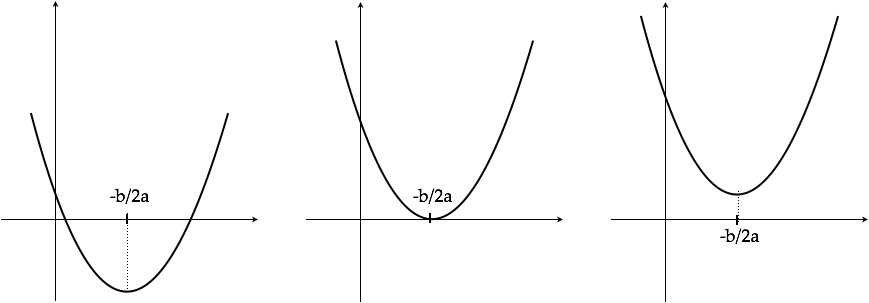
\includegraphics[scale=0.325]{FiguresArithmetic/SecondDegreeInit}
\caption{$P(x)$ has: (left) two real roots; (center) one real root; (right) no real root.}
\label{fig:SecondDegreeInit}
\end{center}
\end{figure}
\begin{itemize}
\item
The solutions $x_1$ and $x_2$ are distinct real numbers.

\smallskip

This corresponds to the lefthand plot in the figure: $P(x)$ crosses the (real) $X$-axis at two distinct points.

\item
The solutions $x_1$ and $x_2$ are identical real numbers.

\smallskip

This corresponds to the central plot in the figure: $P(x)$ crosses/touches the (real) $X$-axis at precisely one point.

\item
The solutions $x_1$ and $x_2$ are distinct {\em non}-real numbers.

\smallskip

This corresponds to the righthand plot in the figure: $P(x)$ never touches the (real) $X$-axis.
\end{itemize}

\ignore{***************
\begin{equation}
\label{eq:generic-quadratic-geo}
P(x) \ = \  ax^2 \ + \ bx \ + \ c \ \ \mbox{  where  } \ b,c \in \R;
\ a \in \R \setminus \{0\}
\end{equation}

Let consider that $a>0$, the case where $a<0$ is symmetric.
Fig.~\ref{fig:SecondDegreeInit} gives an illustration of the possible solutions.


In the case where there are two solutions, we first determine the coordinates of the minimum of $P(x)$.
This is obtained by a simple derivative whose solution is equal to~$x^*=\frac{-b}{2a}$,
the corresponding ordinate is:
\[
%\label{eq:generic-quadratic-1}
y^* \ = \ a.(\frac{-b}{2a})^2 \ + \ b.(\frac{-b}{2a}) \ + \ c \ = \ \frac{-b^2+ 4ac}{4a}
\]

Let $\Delta$ denote the discriminent $b^2 - 4ac$.

From Fig.~\ref{fig:SecondDegree}, the two roots we are looking for are symmetric in regard to $x^*=\frac{-b}{2a}$.
\begin{figure}[htb]
\begin{center}
       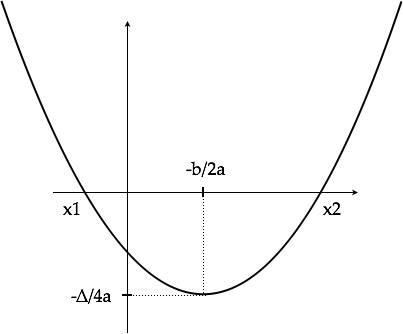
\includegraphics[scale=0.4]{FiguresArithmetic/SecondDegree}
\caption{Geometric interpretation of solving $P(x)=0$.}
\label{fig:SecondDegree}
\end{center}
\end{figure}
******************}


\bigskip

\paragraph{B. Solving cubic polynomials by radicals}

\index{Polynomial!cubic!generic} \index{polynomial!solving a cubic polynomial} 

We derive a formula for the roots of the general cubic polynomial  with real coefficients:
\begin{equation}
\label{eq:generic-cubic-1}
P(x) \ = \  ax^3 \ + \ bx^2 \ + \ cx \ + \ d \ \ \mbox{  where  }
\ b,c, d  \in \R;\ a \in \R \setminus \{0\}
\end{equation}
Although the so-called {\em cubic formula}, which we derive now, is daunting in form, its proof and derivation should be quite accessible because they follow the same flow as the clerically much simpler proof and derivation of the quadratic formula.  For this reason, we derive the 
Because the cubic formula is so complex in form, we present the cubic formula step by step {\em before} we present the formula.

\begin{proof} {\it (Derivation of the cubic formula)}

\smallskip

\noindent {\it Step 1.} Convert $P(x)$ to a {\em monic} cubic polynomial $P^{(1)}(x)$ which shares $P(x)$'s roots.

\smallskip

\noindent
We accomplish this via a change of coefficients that rewrites $P(x)$ as the monic cubic polynomial
\begin{equation}
\label{eq:generic-cubic-2}
P^{(1)}(x) \ = \  x^3 \ + \ Bx^2 \ + \ Cx \ + \ D
\end{equation}
The required change of coefficients is specified implicitly as follows
\[
B \ = \ \frac{b}{a}; \ \ \
C \ = \ \frac{c}{a}; \ \ \
D \ = \ \frac{d}{a}
\]

\medskip

\index{polynomial!cubic!monic!reduced form}

\noindent {\it Step 2.} Convert $P^{(1)}$ to a {\em reduced form} cubic polynomial $P^{(2)}$ which shares $P$'s roots.  By ``reduced'', we mean that $P^{(2)}$ has no quadratic term---i.e., no term in which the variable is raised to the power $2$.

\smallskip

\noindent
We accomplish this transformation as follows.  We make the following change of variable in (\ref{eq:generic-cubic-2}).
\begin{equation}
\label{eq:cubic-substitute-y-for-x} 
y \ = \ x \ + \ \frac{B}{3}
\end{equation}
We thereby convert $P^{(1)}(x)$, a polynomial in variable $x$, into the following polynomial in variable $y$:
\begin{eqnarray}
\nonumber
P^{(2)}(y) & = &  \left(y - \frac{B}{3} \right)^3
 \ + \ B \left(y - \frac{B}{3} \right)^2
 \ + \ C \left(y - \frac{B}{3} \right) \ + \ D \\
\label{eq:generic-cubic-3}
           & = &
y^3 \ + \
\left( \frac{B^2}{9} \ - \ \frac{2B^2}{3} \ + \ C  \right) y
\ + \ \left( \frac{2 B^3}{27}  \ - \ \frac{BC}{3}  \ + \ D \right)
\end{eqnarray}
For simplicity, we rewrite $P^{(2)}(y)$, which clearly is in reduced form, as
\begin{eqnarray}
\label{eq:generic-cubic-4}
P^{(2)}(y) & = & y^3 \ + \ E y \ + \ F \\
\nonumber
\mbox{where} & & \\
\nonumber
E & = & \frac{B^2}{9} \ - \ \frac{2B^2}{3} \ + \ C \\
\nonumber
F & = & \frac{2 B^3}{27}  \ - \ \frac{BC}{3}  \ + \ D
\end{eqnarray}


\medskip

\noindent {\it Step 3.} Convert $P^{(2)}(y)$ to its {\em associated} quadratic polynomial.

\index{Vi\`{e}te, Fran\c{c}ois} \index{Vieta, Franciscus}

\noindent
We accomplish this step by applying a transformation that is attributed to the $16$th-century French mathematician Fran\c{c}ois Vi\`{e}te (often referred to by his Latinized name, Franciscus Vieta) ; see \cite{Hazewinkel}.  Vieta's transformation converts $P^{(2)}(y)$ to a quadratic polynomial by means of the following variable-substitution in (\ref{eq:generic-cubic-4}):
\begin{equation}
\label{eq:cubic-substitute-z-for-y}
y \ = \ z \ - \ \frac{E}{3z}
\end{equation}
We thereby obtain (after calculations involving several cancellations) an expression
\begin{eqnarray}
\nonumber
P^{(3)}(z) & = & \left( z \ - \ \frac{E}{3z} \right)^3
\ + \ E \left(z \ - \ \frac{E}{3z} \right) \ + \ F \\
\label{eq:generic-cubic-5}
  & = &
z^3 \ - \ \frac{E^3}{27z^3}  \ + \ F
\end{eqnarray}
Clearly, $P^{(3)}(z)$ is not a polynomial in $z$---because of the term in which variable $z$ appears in the denominator.  But it is a valuable stepping stone because the function $P^{(3)}(z)$ vanishes---i.e., $P^{(3)}(z) = 0$---precisely when the following polynomial (in the ``variable'' $z^3$) vanishes.
\[ P^{(4)}(z^3) \ = \ (z^3)^2 \ + \ (z^3) F \ - \ \frac{E^3}{27} \]
We wrote both instances of $z^3$ in the expression for $P^{(4)}(z^3)$ within parentheses to facilitate the view of $P^{(4)}(z^3)$ as a (quadratic) polynomial in the ``variable'' $z^3$.  The quadratic formula (\ref{eq:generic-quadratic-4}) provides us with two roots for $P^{(4)}$, which we express as the following two values for $z^3$ (abbreviated via the shorthand operator $\pm$).   \index{$\pm$: plus-or-minus}
\begin{equation}
\label{eq:solve-cubic-for-z3}
(z^3) \ = \
%\frac{1}{2} \left(-F \ \pm \ \sqrt{F^2 + 4 \frac{E^3}{27}} \right) \ = \ 
- \frac{F}{2} \ \pm \ \sqrt{\frac{F^2}{4} + \frac{E^3}{27}}
\end{equation}
We can now derive all solutions for the variable $z$ in equation (\ref{eq:solve-cubic-for-z3}) via back-substitution in transformation (\ref{eq:cubic-substitute-z-for-y}).  But completing this derivation requires a bit of background.

\medskip

\index{Euler's formula} \index{Euler, Leonhard}

Theorem~\ref{thm:fund-thm-algebra} assures us that the polynomial $P^{(2)}(z)$ has three roots.  In order to compute these roots, we invoke a truly remarkable result that is known as  {\it Euler's formula}, in honor of its discoverer, the much-traveled $18$th-century mathematician Leonhard Euler.  This result/formula exposes a fundamental relationship among:
\begin{itemize}
\item
the imaginary unit \index{$i$: the imaginary unit} $i$
\item
the ratio of the circumference of a circle to its radius, $\pi \ = \ 3.141592653 \cdots$
\index{$\pi$: the ratio of the circumference of a circle to its radius}
\item
the base of natural logarithms, Euler's constant $e \ = \ 2.718281828 \cdots$
\index{Euler's constant}\index{$e$:the base of natural logarithms}
\end{itemize}

\begin{theorem}[Euler's formula]
\label{thm:Euler's-formula}
\[ e^{i \pi} \ = \ -1 \]
\end{theorem}

\smallskip

\index{primitive $n$th roots of unity}
  
Back to equation (\ref{eq:solve-cubic-for-z3}): Theorem~\ref{thm:fund-thm-algebra} tells us that within the complex number system $\C$, the cubic polynomial
\[ u^3 \ - \ 1 \]
has three distinct roots.  These numbers are known as the {\em primitive $3$rd roots of unity}  and are traditionally denoted $\omega^0$, $\omega^1$, and $\omega^2$.  Using Theorem~\ref{thm:Euler's-formula}, we can provide explicit values for these numbers:
\[ \omega^0 \ = \ 1; \ \ \ \ \
\omega^1 \ = \ e^{2i \pi/3}; \ \ \ \ \
\omega^2 \ = \ e^{4i \pi/3}.
\]
{\em Aside:} There are analogues of these numbers for any parameter $n$, not just for $n=3$.  For general $n$, the {\it $n$th primitive roots of unity} comprise the set
\[ \{ e^{2ki \pi/n} \ | \ k = 0, 1, \ldots n-1\} \]

\medskip

When we unite the abbreviated double equation (\ref{eq:solve-cubic-for-z3}) for $z^3$ with Euler's formula (Theorem~\ref{thm:Euler's-formula}), we discover {\em six} solutions for the variable $z$, namely, {\small
\begin{equation}
\label{eq:cubic-solution-1}
\begin{array}{ccrrrrrccr}
z_1 & = &
{\displaystyle
\omega^0 \cdot
\left( -\frac{F}{2} \ + \ \sqrt{\frac{F^2}{4} + \frac{E^3}{27}}
\right)^{1/3} 
}
  & & & & &
z_2 & = &
{\displaystyle
\omega^0 \cdot
\left( -\frac{F}{2} \ - \ \sqrt{\frac{F^2}{4} + \frac{E^3}{27}}
\right)^{1/3}
} \\
z_3 & = &
{\displaystyle
\omega^1 \cdot
\left( -\frac{F}{2} \ + \ \sqrt{\frac{F^2}{4} + \frac{E^3}{27}}
\right)^{1/3}
}
  & & & & & 
z_4 & = &
{\displaystyle
\omega^1 \cdot
\left( -\frac{F}{2} \ - \ \sqrt{\frac{F^2}{4} + \frac{E^3}{27}}
\right)^{1/3}
} \\
z_5 & = &
{\displaystyle
\omega^2 \cdot
\left( -\frac{F}{2} \ + \ \sqrt{\frac{F^2}{4} + \frac{E^3}{27}}
\right)^{1/3}
}
  & & & & &
z_6 & = &
{\displaystyle
\omega^2 \cdot
\left( -\frac{F}{2} \ - \ \sqrt{\frac{F^2}{4} + \frac{E^3}{27}}
\right)^{1/3}
}
\end{array}
\end{equation}
}

\smallskip

The algorithmically interesting portion of the process of solving cubics by radicals is now complete.  The remainder of the process consists of ``reversing'' the two transformations,
(\ref{eq:cubic-substitute-z-for-y}) and (\ref{eq:cubic-substitute-y-for-x}), which have taken us from the problem of solving a polynomial in $x$ to the problem of solving a polynomial in $z$.  The calculations that embody this reverse transformation are onerous when solved symbolically, so we make do with some exercises in which the reader will solve numerical instances.  The most interesting and noteworthy feature of these exercises will be the observation of ``collapsing'' of intermediate expressions, whose impact is to leave us with with only {\em three} solutions for $x$---i.e., the number promised by Theorem~\ref{thm:fund-thm-algebra}---rather than the six solutions that the array (\ref{eq:cubic-solution-1}) of $z$-values would lead us to expect.

\smallskip

While the promise of a visually appealing cubic analogue of the quadratic formula (\ref{eq:generic-quadratic-4}) is appealing, the actual cubic formula is so complex visually that it offers no important insights.  The curious reader can find renditions of the formula on the web. \qed
\end{proof}

\subsection{Bivariate Polynomials: The Binomial Theorem}
\label{sec:bivariate-polynomials}
\label{sec:Binomial-thm}
\index{polynomials!bivariate}
\index{The Binomial Theorem}

A polynomial $P$ is {\em bivariate} if each of its summand monomials has the form
\[ a \cdot x^b \cdot y^c \]
In this expression: $x$ and $y$ are the monomial's two variables ({\em two} because the polynomial is {\em bivariate}); $a$ is the monomial's coefficient; $b$ and $c$ are the respective powers of variables $x$ and $y$ in this monomial.

\smallskip

Probably the simplest bivariate polynomials are the ones in the following family.
\begin{equation}
\label{eq:binomial-polys}
\mbox{For } \ n \in \N^+, \ \ \
P_n(x,y) \ \eqdef \ (x+y)^n
\end{equation}
There are lessons to be learned from studying the structure of the polynomials in this family, so let us begin to expand the polynomials using the arithmetic techniques we have learned earlier.
\begin{eqnarray*}
P_1(x,y) \ = \
(x+y)^1 & = & x+y  \\
P_2(x,y) \ = \
(x+y)^2 & = & (x+y) \cdot (x+y) \\
             & = & x^2 + 2xy + y^2 \\
P_3(x,y) \ = \
(x+y)^3 & = & (x+y) \cdot (x^2 + 2xy + y^2) \\
            & = & (x^3 + 2x^2y +  xy^2) + (x^2y + 2xy^2 + y^3) \\
            & = & x^3 + 3x^2y + 3xy^2 + y^3  
\end{eqnarray*}

Let us take a moment to review what we are observing.  We have remarked before that doing mathematics can sometimes involve a wonderfully exciting---and quite sophisticated---pattern-matching game.  So, let us pattern-match!
\begin{enumerate}
\item
The sequence of coefficients of the expanded $P_1(x,y)$ is $\langle 1,1 \rangle$.
\item
The sequence of coefficients of the expanded $P_2(x,y)$ is $\langle 1,2,1 \rangle$.
\item
The sequence of coefficients of the expanded $P_3(x,y)$ is $\langle 1,3,3,1 \rangle$.
\end{enumerate}
There is a familiar pattern emerging here.  Can you spot it?  Where have we seen a pattern of tuples that begins in the same manner?  As a rather broad hint, look at Fig.~\ref{fig:pascal-triangle}!  Could the coefficients of each $P_n$ possibly be the successive binomial coefficients:
\[ {n \choose 0}, \ \ {n \choose 1}, \ \ \ldots, \ \ {n \choose
  {n-1}}, \ \ {n \choose n}
\]
Let us use induction to explore this possibility by expanding a generic $P_n$ with symbolic ``dummy'' coefficients and see what this says about $P_{n+1}$.  To this end, let $a_{n,n-r}$ denote the coefficient of $x^{n-r} y^r$ in the expansion of $P_n(x,y)$.  Using our symbolic coefficients $a_{n,k}$, we have (omitting multiplication symbols to conserve horizontal space):
\begin{eqnarray*}
P_n(x,y) & = &
 x^n \ + \ a_{n,n-1} x^{n-1} y \ + \cdots + \\
         &   & \hspace*{.15in}
a_{n,n-r} x^{n-r} y^r \ + \ a_{n,n-r-1} x^{n-r-1} y^{r+1}
\ + \ a_{n,n-r-2} x^{n-r-2} y^{r+2} \\
         &   & \hspace*{.15in}
+ \cdots + \ a_{n,1} x y^{n-1} \ + \ y^n
\end{eqnarray*}
Continuing with this symbolic evaluation, we have:
\begin{eqnarray}
\nonumber
x \cdot P_n(x,y) & = &
 x^{n+1} \ + \ a_{n,n-1} x^n y \ + \cdots + \\
\nonumber
         &   & \hspace*{.15in}
a_{n,n-r} x^{n-r+1} y^r \ + \ a_{n,n-r-1} x^{n-r} y^{r+1}
\ + \ a_{n,n-r-2} x^{n-r-1} y^{r+2} \\
\label{eq:xPk}
         &   & \hspace*{.15in}
+ \cdots + \ a_{n,1} x^2 y^{n-1} \ + \ x y^n
\end{eqnarray}
and
\begin{eqnarray}
\nonumber
y \cdot P_n(x,y) & = &
 x^n y \ + \ a_{n,n-1} x^n y^2 \ + \cdots + \\
\nonumber
         &   & \hspace*{.15in}
a_{n,n-r} x^{n-r} y^{r+1} \ + \ a_{n,n-r-1} x^{n-r-1} y^{r+2}
\ + \ a_{n,n-r-2} x^{n-r-2} y^{r+3} \\
\label{eq:yPk}
         &   & \hspace*{.15in}
+ \cdots  + \ a_{n,1} x^2 y^n \ + \ y^{n+1}
\end{eqnarray}
Because
\[ P_{n+1}(x+y) \ = \ (x+y) \cdot P_n(x,y) \ = \ x \cdot P_n(x,y) \ + \ y \cdot P_n(x,y) \]
the symbolic coefficient $a_{n-r+1,r}$ of $x^{n-r+1} y^r$ in $P_{n+1}(x+y)$ is the sum of the following symbolic coefficients in $P_n(x,y)$:
\begin{center}
$\bullet$
the coefficient $a_{n,n-r}$ of $x^{n-r}y^r$ \ \ \ \ \
and \ \ \ \ \
$\bullet$
the coefficient $a_{n,n-r+1}$ of $x^{n-r+1}y^{r-1}$
\end{center}
By induction, then, for all $n,r \in \N$ with $r \leq n$,
\[ a_{n,r} + a_{n,r+1} \ = \ a_{n+1,r+1} \]
Combining this equation with the observed initial conditions
\[ a_{1,0} \ = \ a_{1,1} \ = \ 1 \]
we see that each coefficient $a_{n,r}$ is actually the binomial coefficient $\displaystyle {n \choose r}$.

\smallskip

\index{Newton, Isaac}
 
The preceding observation is attributed to the renowned English mathematician/physicist Isaac Newton and is enshrined in Newton's famous {\it Binomial Theorem}.  In fact, the calculations preceding the observation constitute a proof of this seminal result.

\ignore{**********
so that, finally,
\begin{eqnarray*}
             & = &
 x^{k+1} \ + \ (k+1) x^k y \ + \ \cdots \ + \
   (a_{k,k-r-1} + a_{k,k-r}) x^{k-r} y^{r+1} \\
             &   & \ \ \ + \
   (a_{k,k-r-2} + a_{k,k-r-1}) x^{k-r-1} y^{r+2}
 \ + \ \cdots \ + \ (k+1) xy^k \ + \ y^{k+1} \\
      & = &
 x^{k+1} \ + \ (k+1) x^k y \ + \ \cdots \ + \
 a_{k+1,k-r} x^{k-r} y^{r+1} \\
            &    & \ \ \ + \  a_{k+1,k-r-1} x^{k-r-1} y^{r+2}
 \ + \ \cdots \ + \ (k+1) xy^k \ + \ y^{k+1}
\end{eqnarray*}
*******}

\begin{theorem}[The Binomial Theorem]
\label{thm:Binomial-theorem}
For all $n \in \N$,
\begin{equation}
\label{eq:binomial-theorem}
(x+y)^n \ \ = \ \ \sum_{i=0}^n \ \ {n \choose i} x^{n-i} y^i
\end{equation}
\end{theorem}
\index{The Binomial Theorem!binomial coefficients}
\index{binomial coefficients!The Binomial Theorem}
\index{polynomials!bivariate!The Binomial Theorem}


\subsection{$\oplus$ Integer Roots of Polynomials: Hilbert's $10$th Problem}
\label{sec:Hilberts-Tenth}
\index{Hilbert's Tenth Problem}

This section is devoted to describing a true milestone in the history of mathematics, of logic, and of computing.  Even though the mathematical details necessary to fully describe the analyses that lead to this blockbuster theorem go way beyond the scope of an introductory text, this result has cultural lessons that make even its story valuable.  An important source of this value is that the reader who understands even the outlines the theorem will be receptive to the broad implications of the material in Section~\ref{sec:Reals-uncountable}, Section~\ref{sec:pairing}, and Chapter~\ref{Appendix:building-pairing-functions}, which we will come to before too long.  This material supplies essential mathematical underpinnings for the theorem whose tale we are about to embark on.

\medskip

\index{Hilbert, David}  \index{Newson, Mary Frances Winston} \index{Hilbert's Tenth Problem}

In 1900, the eminent, influential German mathematician David Hilbert set forth a list of $23$ problems to serve as a ``bucket list''\footnote{The ``bucket'' is not yet empty.  A number of Hilbert's original $23$ are yet to be solved.}~for the world mathematics community at the dawn of the 20th century.\footnote{Hilbert's list was published in 1902 \cite{Hilbert02}; it was translated into English by Mary Frances Winston Newson, the first American woman to receive a doctorate from the University of G\"{o}ttingen (which was probably the world's premier university for mathematical research in the late 19th and early 20th centuries).}  Of Hilbert's $23$ problems, the $10$th stands out within the world of computing.  Stated in modern terminology, with a modern perspective, the Problem can be stated as follows.
\begin{description}
\item[{\bf Hilbert's Tenth Problem}]
{\it Develop an algorithm that will decide---via a {\sc yes} or {\sc no} answer---whether a given multivariate polynomial with integer coefficients has any integer roots.}
\end{description}
The Problem attracted the attention of many of the best mathematical minds of the 20th century.  Building on the work of American mathematicians Martin Davis and Julia Robinson.  The Problem was finally resolved by the Russian then-graduate student Yuri Matiyasevich.
\index{Davis, Martin} \index{Robinson, Julia} \index{Matiyasevich, Yuri}

\bigskip

\noindent \fbox{ \begin{minipage}{0.96\textwidth}
{\bf Historical note}.

This is certainly not the only instance of a young person making a world-class contribution to mathematics!  Look, for instance, back at our reference to Galois!  The message is clear: Study hard, and aim high!
\end{minipage}
}

\bigskip

\begin{theorem}[Hilbert's Tenth Problem, Resolved]
\label{thm:Hilberts-10th}
There is no algorithm that, when presented with an arbitrary multivariate polynomial $P$ with integer coefficients, will correctly determine whether $P$ has any integer roots.
\end{theorem}

The long history leading to Matiyasevich's proof of Theorem~\ref{thm:Hilberts-10th} is documented in \cite{Davis73,DavisH73,DavisMR76,Matiyasevich93}.  The first three of these sources give accessible, informal descriptions of the exciting journey from Hilbert to Matiyasevich.

\medskip

The mathematics needed even to understand Hilbert's Tenth Problem and its resolution are beyond an introductory text.  However, a few words are in order about the exciting way in which Theorem~\ref{thm:Hilberts-10th} fundamentally changed the course of 20th-century mathematics by turning the table on all of the mathematics that had been done to that point in history.

\medskip

We recall from Section~\ref{sec:classical-v-modern-proofs} that one of the main movements that took root in 19th-century mathematics had as its goal to codify the notion of ``rigorous proof''.  Toward this end, one of Hilbert's goals in his to-do list of 1900---especially with regard to the 10th problem on his list---was to have mathematicians rigorously prove that the notions of ``Truth'' and ``Provability'' coincided.  Hilbert's immediate challenge was to find such a proof at least for ``elementary'' areas of mathematics.

\smallskip

\index{G\"{o}del, Kurt} \index{G\"{o}del's Incompleteness Theorems}

This hope was, in fact, the first of Hilbert's dreams to be dashed: In the early 1930s, Austrian expatriate, then Princeton professor, Kurt G\"{o}del, proved the first of his celebrated {\it Incompleteness Theorem}s \cite{Goedel31}.  Stated {\em very(!)}~informally, this first theorem asserts that in any ``reasonable'' mathematical system, there will always be {\em true} statements that cannot be proved.

\bigskip

\noindent \fbox{
\begin{minipage}{0.96\textwidth}
{\bf Explanatory note}.

Two crucial words remain unspecified in our story, namely, ``elementary'' and ``reasonable''.  Both refer to what is, intuitively, the simplest domain in formal mathematics---the study of the basic properties of positive integers.  Specifically, both words point to a mathematical system which is capable of dealing with elementary assertions about triples, $x, y, z$, of positive integers, specifically, the following assertions:
\begin{itemize}
\item
One given integer, say $z$, is the sum of the other two ($z = x+y$).
\item
One given integer, again say $z$, is the product of the two others ($z = x \times y$).
\end{itemize}
\end{minipage}
}

\bigskip

\index{Turing, Alan} \index{uncomputable function} \index{Cantor, Georg}

\noindent
Building on G\"{o}del's insights, English mathematician Alan Turing soon thereafter proved---again, stated {\em very(!)}~informally---that no matter how much ``smarts'' we build into a digital computer using digital logic, there will always be functions---even $0$-$1$ valued functions---that the computer cannot compute \cite{Turing36}.  Theorem~\ref{thm:Hilberts-10th} can be reworded to assert that the integer-root-finding behavior called for in Hilbert's Tenth Problem is one of Turing's {\it uncomputable} functions!\footnote{The connections between G\"{o}del's work and Turing's, and the manner in which both authors' work connects to the work of German logician Georg Cantor  on infinite sets of numbers, \cite{Cantor74,Cantor78} are described in \cite{Rosenberg09} using consistent terminology to discuss all three authors' work.}


\section{Exponential and Logarithmic Functions}
\label{sec:exponential+logarithm}

This section introduces the fundamentals of the mathematically and computationally important functions that emerge from the operations of exponentiation and taking logarithms.  These functions are mutually inverse, in the sense of equation (\ref{eq:functional-inverse}).

\subsection{Basic Definitions}
\label{sec:exponential-function}

\index{exponential function} \index{function!exponential}

A function $f$ is {\it exponential} if there is a positive number $b$ such that, for all $x$,
\begin{equation}
\label{eq:exponential-defn}
f(x) \ = \ b^x
\end{equation}
The number $b$ is the {\it base}\index{base of exponential} of function $f(x)$.  The basic arithmetic properties of exponential functions are easily derived from the recurrent system of equations (\ref{eq:power-def}).  The important message is that multiplication ``at the ground level'' is addition at the ``exponent level'':
\[ b^x \times b^y \ = \ b^{x+y} \]

\index{logarithmic function} \index{base-$b$ logarithm} \index{function!logarithmic}
\index{$\log_b a$: the base-$b$ logarithm of number $a$}

Given an integer $b >1$ (mnemonic for ``base''), the {\em base-$b$ logarithm} of a real number $a > 0$ is denoted $\log_b a$ and defined by the equation
\begin{equation}
\label{eq:logarithm-defn}
a \ = \ b^{\log_b a}
\end{equation}
Logarithms are partial functions: $\log_b a$ is not defined for non-positive values of $a$.

\smallskip

\index{$\log(a)$: base-$2$ logarithm of number $a$}
\index{$\ln(a)$: base-$2$ logarithm of number $a$}. 

The base $b = 2$ is so prominent in the contexts of computation theory and information theory that we commonly invoke one of two special notations for $\log_2 a$: (1) we often elide the base-$2$ subscript and write $\log a$; (2) we employ the specialized notation $\ln a$.  Notationally:
\[ \log_2 a \ \eqdef \ \log a \ \eqdef \ \ln a \]

\smallskip

We leave to the reader the easy verification, from (\ref{eq:logarithm-defn}), that the {\it base-$b$ logarithmic function}, defined by
\begin{equation}
\label{eq:log-function-defn}
f(x) \ = \ \log_b x
\end{equation}
is the functional inverse of the base-$b$ exponential function.

\subsection{Learning from Logarithms (and Exponentials)}

Definition (\ref{eq:logarithm-defn}) exposes and---even more importantly---explains myriad facts about logarithms, which we often take for granted.

\begin{prop}
\label{thm:log-add-multiply}
For any base $b >1$, for all numbers $x >0$, $y>0$,
\[ \log_b (x \cdot y) \ = \ \log_b x \ + \ \log_b y \]
\end{prop}

\begin{proof}
Definition (\ref{eq:logarithm-defn}) tells us that $x = b^{\log_b x}$ and $y = b^{\log_b y}$.  Therefore,
\[ x \cdot y \ = \ b^{\log_b x} \cdot b^{\log_b y} \ = \
b^{\log_b x \ + \ \log_b y} \]
by the laws of powers.  Taking base-$b$ logarithms of the first and last terms in the chain yields the claimed equation.  \qed
\end{proof}

\medskip

\index{slide rule}

\noindent \fbox{\begin{minipage}{0.96\textwidth}
{\bf Historical note}.

Proposition~\ref{thm:log-add-multiply} provides the mathematical underpinnings of the analogue computing device known as a {\it slide rule}.  Without going into details, a slide rule is built from two straight sticks that are both marked off according to a logarithmic scale.  The sticks are attached in a way that allows each to slide along the other (whence the name of the device); see Fig.~\ref{fig:slide-rule}.
The important property of this device is illustrated in the figure:  When one positions the origin (number $1$ of stick $A$ at the position of stick $B$ that corresponds to number $a$, then the number on stick $B$ that corresponds to the number $b$ on stick $A$ is $a \times b$.  In short, the logarithmic scale on the device's sticks enables it to translate linear motion (the sliding of the sticks relative to one another) into numerical multiplication.
\end{minipage}
}

\begin{figure}[htb]
\[ 
\begin{array}{|c|}
\hline
\begin{array}{ll}
A \hspace*{.35in} &
\hspace*{.35in}
\fbox{$1$ \hspace*{.3in} \fbox{$b$} 
\hspace*{.7in} $2$ 
\hspace*{.5in} $3$ 
\hspace*{.25in} $4$ 
\hspace*{.125in} $5$} \\ 
  &
\hspace*{.4in} \updownarrow \hspace*{.41in} \updownarrow \\
B \hspace*{.35in} &
\fbox{$1$\hspace*{.24in}\fbox{$a$}\hspace*{.25in}\fbox{$a \cdot b$}
\hspace*{.3in} $2$ 
\hspace*{.5in} $3$ 
\hspace*{.25in} $4$ 
\hspace*{.125in} $5$}
\end{array}
 \\
\hline
\end{array}
\]
\caption{A schematic view of a slide rule performing a multiplication.  If one slides Stick $A$ to position $a$ of Stick $B$, then position $b$ of Stick $A$ appears directly above position $a \cdot b$ of Stick $B$.  Thereby, the addition of distances on the rule's logarithmic scale is used to compute products.}
\label{fig:slide-rule}
\end{figure}


\bigskip

\noindent
Many people believe that the following important property of logarithms is a {\em convention} rather than a consequence of the basic definitions:
\smallskip

 {\em The logarithm of $1$ to any base is $0$.}

\smallskip

\noindent We correct this misapprehension now.

\smallskip

\begin{prop}
\label{thm:log1=0}
For any base $b >1$,
\[ \log_b 1 \ = \ 0 \]
\end{prop}

\begin{proof}
We note the following chain of equalities.
\[  b^{\log_b x} \ = \ b^{\log_b (x \cdot 1)} 
  \ = \ b^{(\log_b x) + (\log_b 1)} 
  \ = \ b^{\log_b x} \cdot b^{\log_b 1}
\]
Hence, $b^{\log_b 1} \ = \ 1$.  If $\log_b 1$ did not equal $0$, then $b^{\log_b 1}$ would exceed $1$.  \qed
\end{proof}

Similar exploitation of the basic definitions yields the following fundamental properties of logarithms (to any base).

\begin{prop}
For all bases $b > 1$ and all numbers $x, y$,
\[ x^{\log_b y} \ = \ y^{\log_b x} \]
\end{prop}

\begin{proof}
We invoke (\ref{eq:logarithm-defn}) twice to remark that
\[ \left[x^{\log_b y} \ = \ b^{(\log_b x) \cdot (\log_b y)}\right]
\ \ \mbox{ and } \ \ 
\left[y^{\log_b x}\ = \ b^{(\log_b y) \cdot (\log_b x)}\right] \]
The commutativity of addition completes the verification.  \qed
\end{proof}

\smallskip

\begin{prop}
For any base $b >1$,
\[ \log_b (1/x) \ = \ - \log_b x \]
\end{prop}

\begin{proof}
By the product law for logarithms,
\[ \log_b x + \log_b (1/x) \ = \ \log_b (x \cdot (1/x))
\  = \ \log_b 1
\]
An invocation of Proposition~\ref{thm:log1=0} completes the proof.  \qed
\end{proof}

\smallskip

\begin{prop}
For any bases $a, b >1$,
\begin{equation}
\label{eq:log-exp-0}
\log_b x \ = \ \left(\log_b a \right) \cdot \left( \log_a x \right)
\end{equation}
\end{prop}

\begin{proof}
We begin by noting that, by definition,
\begin{equation}
\label{eq:log-exp-1}
 x \ = \ b^{\log_b x} \ = \ a^{\log_a x}
\end{equation}
We now take the base-$b$ logarithm of the second and third expressions in (\ref{eq:log-exp-1}) and then invoke the product law for logarithms.  The second expression tells us that
\begin{equation}
\label{eq:log-exp-2}
 \log_b \left(b^{\log_b x} \right) \ = \ \log_b x
\end{equation}
The third expression tells us that
\begin{equation}
\label{eq:log-exp-3}
 \log_b \left( a^{\log_a x} \right) \ = \
\left(\log_b a \right) \cdot \left( \log_a x \right)
\end{equation}
We know from the double equation (\ref{eq:log-exp-1}) that the righthand expressions in equations (\ref{eq:log-exp-2}) and (\ref{eq:log-exp-3}) are equal.  Equation (\ref{eq:log-exp-0}) follows by transitivity.  \qed
\end{proof}

\noindent
By setting $x = b$ in equation (\ref{eq:log-exp-0}), we discover the following marvelous equation.

\begin{prop}
For any integers $a, b >1$,
\begin{equation}
\left(\log_b a \right) \cdot \left( \log_a b \right) \ = \ 1 \ \ \ \ \
\mbox{ or, equivalently, } \ \ \ \ \
\log_b a \ = \ \frac{1}{\log_a b} 
\end{equation}
\end{prop}


\section{$\oplus$ Pointers to Specialized Topics}

Emerging technologies prolifically give rise to novel specialties that grab the imagination of the computer-literate public.  Since many such specialties build upon mathematical concepts and tools, they afford the designer of a mathematics course an opportunity to add enrichment to a syllabus that is dominated by the ``classics.''  During the first decades of the 21st century, application areas such as {\it robotics} or {\it data science} or {\it data mining} or {\it computer security} or {\it energy-awareness} each can benefit from supplements to a standard mathematics syllabus---of course, at levels consistent with the students' preparation.  We now flesh out this suggestion by discussing two supplements which, broadly construed, could fit under the mantle of {\it Arithmetic}.

\subsection{Norms and Metrics for Tuple-Spaces}
\label{sec:Ln-norms}

\index{tuple-spaces}

By the 1950s, computers had become sophisticated enough to handle structured data, computer users became sophisticated enough to think in terms of structured models.  Thus, from the 1960s and 1970s onward to the present, one sees {\it tuple-spaces} used to algorithmic advantage in application areas as varied as {\it databases} \cite{Codd70}, {\it parallel computing} \cite{BlumS77,Shinahr74}, and {\it robotics} \cite{Marchese96,Rosenberg12}.  While the specific concepts drawn from the study of tuple-spaces vary a bit from one application area to another, certain concepts recur---and among these, the {\it norms} and {\it metrics} that allow us to talk about notions such as ``distance'' play a very important role.  Of course, notions of ``distance''
relevant to databases may differ from those used in, e.g., robotic path planning, but in very many applications it is important to know whether tuple $t_1$ is ``closer to'' tuple $t_2$ than to tuple $t_3$.

\smallskip

\index{Lebesgue, Henri L\'{e}on} \index{Lebesgue's $L$-measures}

It is an often-frustrating phenomenon that new application areas all too frequently rename concepts and tools that it inherits from its predecessors.  So how shall we name the norms and metrics that we inject into our mathematics curriculum?  Probably the most scholarly course is to employ the names that honor the early 20th century French mathematician and function theorist Henri L\'{e}on Lebesgue whose $L$-measures form the classical taxonomy of norms and distances in tuple-spaces.

We focus on {\em two-dimensional} tuple-spaces, although everything we say generalizes in a straightforward manner to arbitrary finite-integer dimensionalities.  And, we restrict attention to the three $L$-measures that are the most common in application areas such as informatics and robotics.  Focus on arbitrary $2$-tuples of numbers $z_1 = \langle x_1, y_1 \rangle$ and $z_2 = \langle x_2, y_2 \rangle$.

\medskip

\index{$L^1$ measure} \index{$L^1$ measure!norm} \index{$L^1$ measure!distance}
\index{Manhattan distance} \index{rook distance} \index{NEWS compass directions}

\noindent {\it The $L^1$ measure.}
\begin{itemize}
\item
The $L^1$-{\it norm} of $z_1$ is the sum of the magnitudes of its coordinates, i.e.,
\[ L^1(z_1) \ = \ |x_1| + |y_1|  \]  

\item
The $L^1$-{\it distance} between $z_1$ and $z_2$ is the sum of the magnitudes of the differences between the coordinates of the two pairs, i.e.,
\[ L^1(z_1, z_2) \ = \ |x_1 - x_2| + |y_1 - y_2| \]
\end{itemize}
The $L^1$-distance is also called {\it Manhattan distance} or {\it rook distance}, because a path between $z_1$ and $z_2$, viewed as points in $2$-dimensional space, in which adjacent points are unit $L^1$-distance apart, follows a rectilinear grid-like pattern such one observes in a map of Manhattan or in the path taken by a rook in chess.  From a less picturesque point of view, one observes that each point in $2$-dimensional space is unit $L^1$-distance from four other points, one each in the four NEWS (north, east, south, west) compass directions.  If one maps out the points in $2$-dimensional space that are at successive $L^1$-distances from a ``center'' point $z$, then one observes the {\it $L^1$-disc} of Fig.~\ref{fig:Ln-discs}(left), which generalizes in higher dimensions to the {\it $L^1$-sphere}. \index{$L^1$ measure!sphere} 
\index{$L^1$ measure!disc} 
\begin{figure}[hbt]
\[
\begin{array}{ccc}
\begin{array}{|ccccccc|}
\hline
  &   &   & \fbox{3} &   &   &   \\
  &   & \fbox{3} & \fbox{2} & \fbox{3} &   &   \\
  & \fbox{3} & \fbox{2} & \fbox{1} & \fbox{2} & \fbox{3} &   \\
\fbox{3} & \fbox{2} & \fbox{1} & \fbox{0} & \fbox{1} & \fbox{2} & \fbox{3} \\
  & \fbox{3} & \fbox{2} & \fbox{1} & \fbox{2} & \fbox{3} &   \\
  &   & \fbox{3} & \fbox{2} & \fbox{3} &   &   \\
  &   &   & \fbox{3} &   &   &   \\
\hline
\end{array}
  & \hspace*{.5in} &
\begin{array}{|ccccccc|}
\hline
\fbox{3} & \fbox{3} & \fbox{3} & \fbox{3} & \fbox{3} & \fbox{3} & \fbox{3} \\
\fbox{3} & \fbox{2} & \fbox{2} & \fbox{2} & \fbox{2} & \fbox{2} & \fbox{3} \\
\fbox{3} & \fbox{2} & \fbox{1} & \fbox{1} & \fbox{1} & \fbox{2} & \fbox{3} \\
\fbox{3} & \fbox{2} & \fbox{1} & \fbox{0} & \fbox{1} & \fbox{2} & \fbox{3} \\
\fbox{3} & \fbox{2} & \fbox{1} & \fbox{1} & \fbox{1} & \fbox{2} & \fbox{3} \\
\fbox{3} & \fbox{2} & \fbox{2} & \fbox{2} & \fbox{2} & \fbox{2} & \fbox{3} \\
\fbox{3} & \fbox{3} & \fbox{3} & \fbox{3} & \fbox{3} & \fbox{3} & \fbox{3} \\
\hline
\end{array}
\end{array}
\]
\caption{The radius-$3$ $L^1$-disc (left) and $L^\infty$-disc (right), with annotated $L^1$-distances and $L^\infty$-distances, respectively, from the ``center'' point.}
\label{fig:Ln-discs}
\end{figure}

\medskip

\index{$L^\infty$ measure!norm} \index{$L^\infty$ measure}
\index{$L^\infty$ measure!distance} \index{king's-move distance}

\noindent{\it The $L^\infty$ measure.} 
\begin{itemize}
\item
The $L^\infty$-{\it norm} of $z_1$ is the larger of the magnitudes of its coordinates, i.e.,
\[ L^\infty(z_1) \ = \ \max(|x_1|, \ |y_1|)  \]  

\item
The $L^\infty$-{\it distance} between $z_1$ and $z_2$ is the larger of the magnitudes of the
differences between the coordinates of the two pairs, i.e.,
\[ L^\infty(z_1, z_2) \ = \ \max(|x_1 - x_2|, \  |y_1 - y_2|) \]
\end{itemize}
$L^\infty$-distance is also called {\it king's-move distance}, because each step in a path between $z_1$ and $z_2$, in which adjacent points are unit $L^\infty$-distance apart follows a pattern such as one observes in a path taken by a king in chess.  From a less picturesque point of view, one observes that each point in $2$-dimensional space is unit $L^\infty$-distance from eight other points, one each in the eight compass directions, N, NE, E, SE, S, SW, W, NW.  If one maps out the points in $2$-dimensional space that are at successive $L^\infty$-distances from a ``center'' point $z$, then one observes the {\it $L^\infty$-disc} of Fig.~\ref{fig:Ln-discs}(right), which generalizes in higher dimensions to the {\it $L^\infty$-sphere}.
 \index{$L^\infty$ measure!sphere} \index{$L^\infty$ measure!disc}

\smallskip

As one observes in Fig.~\ref{fig:Ln-discs}, the structures of the $L^1$-disc and the $L^\infty$-disc are, respectively, dominated by diagonals and squares; see the ``equipotential'' lines in the figure.  One can exploit this fact when crafting algorithms that are governed by these norms.  Indeed, we invoke the structures of these discs as we develop the ``pairing functions'' that we showcase in Section~\ref{sec:building-pairing-functions}.

\bigskip

\index{Euclid!{\it The Elements}}

We have not (yet) mentioned what is likely the most familiar $L$-measure, namely, the $L^2$ measure which is named for Euclid in honor of his celebrated treatise on geometry, {\it The Elements}.  For completeness, we now define this measure, but we do not develop the subject further because it is not frequently used when dealing with the discrete mathematical structures
that are the primary foci of this text.

\medskip

\index{$L^2$ measure!norm}  \index{$L^2$ measure} \index{origin of $2$-dimensional space}

\noindent{\it The $L^2$ measure.}
\begin{itemize}
\item
The $L^2$-{\it norm} of $z_1$ is the Euclidean distance of the point from the {\it origin} of
$2$-dimensional space, which is the point $\langle 0,0 \rangle$:
\[ L^2(z_1) \ = \ \sqrt{x_1^2 + y_1^2}  \]  

\item
The $L^2$-{\it distance} between $z_1$ and $z_2$ is the Euclidean distance between the points in $2$-dimensional space, i.e.,
\[ L^2(z_1, z_2) \ = \ \sqrt{(x_1 - x_2)^2 + (y_1 - y_2)^2} \]
\end{itemize}
\index{$L^2$ measure!distance}

\subsection{Edit-Distance: Measuring Closeness in {\em String Spaces}}

From the earliest days of digital computing, the challenge of employing computers as ``editorial assistants'' was viewed as a prime domain within which to achieve a significant practical payoff.  An early problem within this domain was to determine of ``how different'' two strings, $x$ and $y$, composed of letters from an alphabet $A$, are from one another.  The quotation marks in the preceding sentence acknowledge that it is actually not obvious how to measure the ``distance'' between $x$ and $y$ in a way that matters.  The intersecting needs of three separate developing communities finally supplied the definition that has generally been accepted.  Roughly contemporaneously, during the decade from 1955--1965:
\index{Oettinger, Anthony G.} \index{Hopper, Grace Murray} \index{Sammet, Jean E.}
\index{Yngve, Victor} \index{Backus, John}
  \begin{itemize}
  \item
Computational linguists attempted to enlist computers in the processing of natural language.  The goal of automatic translation between Russian and English became the ``holy grail'' of this community, at least in the US and USSR.  Reminiscences by Anthony G.~Oettinger,  a pioneer in this effort, appear in \cite{Hutchins00}.
   \item
As the quickly growing power of computers became appreciated, more sophisticated process-specification languages began to emerge.  From the very early days of this development, programming languages became more ``natural"-language-like.  (There was a split among computer-language designers:  Some interpreted ``natural" as in the phrase ``natural language":  They wanted to program in [an approximation to] English or French or Russian or \ldots.  Others interpreted ``natural" as a synonym for ``problem-specific".  They wanted scientists to be able to feed computers systems of equations, while engineers might feed some textual encoding of a circuit design.) One of the earliest entrants in this arena was the business-oriented language COBOL, which was inspired by early work of the computing giant Grace Murray Hopper and developed under the leadership of Jean E.~Sammet; see \cite{Sammet78}.  A second early entrant was the string-processing language COMIT developed under the leadership of Victor Yngve, with an eye toward applications such as language processing; see \cite{Yngve}.  A champion by any metric was the ever-evolving FORTRAN language which was developed in the mid-1950s by a small team at IBM, headed by John Backus; see \cite{Backus-etal57}.  FORTRAN was the first programming language which aimed to enable scientists to specify the problems they wished to compute in a manner that was at least reminiscent of the mathematical notation they would use to communicate with one another.
   \item
As it became clear that FORTRAN was a step toward satisfying the programming needs of an enormous market, a veritable army of systems programmers began to develop increasingly sophisticated processors for its genre of programming language.  The era of ``smart compilers'' was dawning.
   \end{itemize}

A common feature in the preceding developments was that people were typing more as they used computers.  Inevitably, therefore, they were making more typing mistakes.  A very specific computing challenge arose, to make much more concrete the desire to understand how close a
string $x$ was to a string $y$.  Could one develop an algorithm that would rewrite one of these strings as the other while ``editing'', or, rewriting, as few symbols as possible?  While such an algorithm would not completely solve the ``mistyping'' problem---consider, e.g., that the strings

\hspace*{.25in} ``SORTH'' \ \ and \ \ ``NOUTH''

\noindent
are both ``edit-distance $1$'' from both

\hspace*{.25in} ``SOUTH'' \ \ and \ \ ``NORTH''

\noindent
hence cannot be ``corrected'' automatically---being able to correct a mistyped string to its edit-nearest legitimate string would probably be very useful in practice.  Happily, although this algorithmic problem was more difficult than many had imagined, it did admit the efficient, elegant solution that appears in \cite{WagnerF74}.


%%%%%%%%%%%%%%%%%%%%%%%%%%%%%%%%

\section{Exercises: Chapter 5}

Throughout the text, we mark each exercise with 0 or 1 or 2 occurrences of the symbol $\oplus$, as a rough gauge of its level of challenge.  The 0-$\oplus$ exercises should be accessible by just reviewing the text.  We provide {\em hints} for the 1-$\oplus$ exercises; Chapter~\ref{ch:Exercises} provides {\em solutions} for the 2-$\oplus$ exercises.  Additionally, we begin each exercise with a brief explanation of its anticipated value to the reader.
 
\begin{enumerate}
\item
{\bf Additive and multiplicative identities are unique}

{\sc Lesson:} Enhance familiarity with basic arithmetic argumentation

\smallskip  

{\em Prove the following assertions about $0$ and $1$.}

\begin{prop}
The numbers $0$ and $1$ play unique roles:
\begin{enumerate}
\item
$0$ is the unique additive identity: $(\forall \ n) \ [n+0 = 0 + n = n]$.
\item 
$1$ is the unique multiplicative identity: $(\forall \ n) \ [n \cdot 1 = 1 \cdot n = n]$.
\item
$0$ is the unique multiplicative annihilator: $(\forall \ n) \ [n \cdot 0 = 0 \cdot n = n]$
\end{enumerate}
\end{prop}

\item
{\bf Additive and multiplicative inverses are unique}

{\sc Lesson:} Enhance familiarity with basic arithmetic argumentation

\smallskip  

{\em Prove the following assertions.}

\begin{prop}
\label{thm:AR-EX-mult-inv}
Additive and multiplicative inverses are unique:
\begin{enumerate}
\item
For each number $x$ in $\N$, or in $\Q$, or in $\R$, there is a unique number $y$ in the same class such that $x + y = 0$.
\item 
For each {\em nonzero} number $x$ in $\Q$ or in $\R$, there is a unique number $y$ in the same class such that $x \cdot y = 1$.
\end{enumerate}
\end{prop}

The class $\N$ is (intentionally) missing from Proposition~\ref{thm:AR-EX-mult-inv}.b: integers other than $\pm 1$ do not have integral multiplicative inverses.  We shall take some of the sting out of this lack in 
Section~\ref{sec:EX-NUM2} by means of Proposition~\ref{thm:NUM2-EX-CXL}, which shows that integers have a rudimentary version of multiplicative inverse.

\item
{\bf Verifying the critical properties of rational arithmetic}

{\sc Lessons:} Rational arithmetic works the way that it should.

\smallskip

{\em Prove the following properties of rational arithmetic (``RA" for short):}
\begin{itemize}
\item
{\em RA works correctly when the argument rational numbers are, in fact integers;}
\item
{\em RA treats the number $0$ appropriately, as both an additive identity and a multiplicative annihilator;}
\item
{\em RA treats the number $1$ appropriately, i.e., as a multiplicative identity;}
\item
{\em RA obeys the laws outlined in Section~\ref{sec:Arithmetic-Laws}.}

\smallskip

Verifying the distributivity of rational multiplication over rational addition is an especially valuable exercise because of the amount of manipulation that the verification demands.
\end{itemize}

\item
{\bf Roots of polynomials}

{\sc Lesson:} Practice with roots and polynomial manipulation

{\em Prove the following assertion, which employs the notation of the chapter.}
\begin{prop}
The polynomial
\[ P_1(x) \ \ = \ \ a_d x^d \ + \ a_{d-1} x^{d-1} \ + \ a_{d-2} x^{d-2}
\ + \cdots + \ a_1 x \ + \ a_0
\]
and the monic polynomial
\[ P_2(x) \ = \
x^d \cdot \left( 1 \ + \ \frac{a_{d-1}}{x} \ + \ \frac{a_{d-2}}{x^2}
\ + \cdots + \ \frac{a_1}{x^{d-1}} \ + \ \frac{a_0}{x^d} \right)
\]
have the same roots.
\end{prop}


\item
{\bf Polynomials' degrees and asymptotic growth rates}

{\sc Lesson:} Practice with asymptotic arguments

\smallskip

Let us be given polynomials with positive coefficients: $P(x)$ of degree $a$ and $Q(x)$ of degree $b > a$.  The numbers $a$ and $b$ need not be integers. 

\smallskip

{\em Prove that there exists a constant $X_{P,Q}$---i.e., a constant that depends on the degrees and coefficients of polynomials $P$ and $Q$---such that}
\[ (\forall \ x > X_{P,Q}) \ \left[ P(x) < Q(x) \right] \]

\smallskip

The preceding formulation can be rephrased in the following two ways:

(1) Polynomial $Q$ {\em eventually majorizes} polynomial $P$.

(2) Polynomial $Q$ {\em grows asymptotically faster than} polynomial $P$.

\item
{\bf Exponentials grow asymptotically faster than polynomials}

{\sc Lesson:} Practice with asymptotic arguments

\smallskip

Let us be given a degree-$b$ polynomial $Q$ with positive coefficients, together with an arbitrary real number $c > 1$.

\smallskip

{\em Prove that there exists a constant $Y_{c;Q}$---i.e., a constant that depends on the constant $c$ and on the degree and coefficients of polynomial $Q$---such that}
\[ (\forall \ x > Y_{c,Q}) \ \left[ c^x > Q(x) \right] \]

\item
{\bf Logarithmic functions and exponential functions}

{\sc Lesson:} Taking logarithms and exponentiating are mutually inverse operations

\smallskip

{\em Prove the following assertion.}

\begin{prop}
The base-$b$ logarithmic function
\[ f(x) \ = \ \log_b x \]
and the base-$b$ exponential function
\[ g(x) \ = \ b^x \]
are functional inverses of each other.
\end{prop}

\end{enumerate}

\ignore{************
\subsection{Revisiting a very old problem}

\noindent \textit{The problem.}

The proposed exercice comes from babylonians in the 18th century BC.
Solve the second degree equation $x^2 + x = 45$. where the numbers are expressed in base numeral $60$. 
\medskip

\noindent \textit{Hint.}
The idea of the proof is to represent graphically the equation,
more precisely, the left hand side is represented by the square $x^2$ plus a rectangle $60 \times x$.
Then, the problem is to determine the length of the side of this large rectangle.
\medskip

\noindent \textit{Lesson learned:}
Handling calculations in a non standard basis and provide a geometric solution. 
***************}

